\setcounter{dang}{0}
\setcounter{ex}{0}
\section{Mức độ 7,8 điểm}
\Opensolutionfile{ans}[ans/CD5/Muc_7_8]
\begin{dang}{Xét dấu của các hệ số hàm số thông qua đồ thị}
\end{dang}
\begin{ex}%Câu 1.%[2D1B5-1]
	[Đề Minh Họa 2020 Lần 1]
	\immini
	{
		 Cho hàm số $y=ax^3+3x+d(a;d\in\mathbb{R})$ có đồ thị như hình bên. Mệnh đề nào dưới đây đúng?	
	\choice
	{$a>0,d>0$}
	{$a<0,d>0$}
	{$a>0,d<0$}
	{\True $a<0,d<0$}
	}{
		\begin{tikzpicture}[scale=0.8, font=\footnotesize, line join=round, line cap=round,>=stealth]
			\def\a{-0.7}  % Hệ số co dãn
			\def\xmin{-3} \def\xmax{3}
			\def\ymin{-4} \def\ymax{2} 
			\draw[->] (\xmin,0)--(\xmax,0) node [below]{$x$};
			\draw[->] (0,\ymin)--(0,\ymax) node [left]{$y$};
			\node at (0,0) [below left]{$O$};
			\clip (\xmin+0.1,\ymin+0.1) rectangle (\xmax-0.1,\ymax-0.1);
			\draw[smooth,samples=300] plot(\x,{\a*((\x+2.2)*(\x-0.5)*(\x-1.8))});
		\end{tikzpicture}
	}
	\loigiai{
		Ta có: $\lim\limits_{x\to+\infty}y=-\infty\Rightarrow$ đồ thị nhánh ngoài cùng của hàm số hướng đi xuống nên hệ số $a<0$.\\
		Giao điểm của đồ thị hàm số với trục tung $Oy\colon x=0$ là điểm nằm bên dưới trục hoành nên khi $x=0\Rightarrow y=d<0$.}
\end{ex}
\begin{ex}%Câu 2.%[2D1B5-1]
	[Đề Tham Khảo 2020 Lần 2] Cho hàm số $f(x)=\dfrac{ax+1}{bx+c}\left(a,b,c\in\mathbb{R}\right)$ có bảng biến thiên như sau 
	\begin{center}
		
\begin{tikzpicture}
			\tkzTabInit[nocadre=false,lgt=1.2,espcl=2.5,deltacl=0.6]
			{$x$ /0.6,$f'(x)$ /0.6,$f(x)$ /2}
			{$-\infty$,$2$,$+\infty$}
			\tkzTabLine{,+,d,+,}
			\tkzTabVar{-/$1$,+D-/$+\infty$/$-\infty$,+/$1$}
		\end{tikzpicture}
	\end{center}
	Trong các số $a$, $b$ và $c$ có bao nhiêu số dương?
	\choice
	{$2$}
	{$3$}
	{\True $1$}
	{$0$}
	\loigiai{
		Hàm số $f(x)=\dfrac{ax+1}{bx+c}$ có đường tiệm cận đứng là đường thẳng $x=-\dfrac{c}{b}$ và đường tiệm cận ngang là đường thẳng $y=\dfrac{a}{b}$.\\
		Từ bảng biến thiên ta có: $\heva{&-\dfrac{c}{b}=2\\&\dfrac{a}{b}=1}\Leftrightarrow a=b=-\dfrac{c}{2} (1)$.\\
		Mặt khác: $f'(x)=\dfrac{ac-b}{(bx+c)^2}$.\\
		Vì hàm số đã cho đồng biến trên các khoảng $(-\infty;2)$ và $(2;+\infty)$ nên.\\
		$f'(x)=\dfrac{ac-b}{(bx+c)^2}>0\Leftrightarrow ac-b>0 (2)$.\\
		Thay $(1)$ vào $(2)$, ta được: $-\dfrac{c^2}{2}+\dfrac{c}{2}>0\Leftrightarrow-c^2+c>0\Leftrightarrow 0<c<1$.\\
		Suy ra $c$ là số dương và $a$, $b$ là số âm.}
\end{ex}
\begin{ex}%Câu 3.%[2D1B5-1]
	[Mã 101 - 2020 Lần 1] 
	\immini{
		Cho hàm số $y=ax^3+bx^2+cx+d\left(a,b,c,d\in\mathbb{R}\right)$ có đồ thị là đường cong trong hình bên. Có bao nhiêu số dương trong các số $a$, $b$, $c$, $d$?
	\choice
	{$4$}
	{$1$}
	{\True $2$}
	{$3$}
	}{
		\begin{tikzpicture}[scale=1, font=\footnotesize, line join=round, line cap=round,>=stealth]
			\def\a{-0.7}  % Hệ số co dãn
			\def\xmin{-1.5} \def\xmax{5}
			\def\ymin{-1} \def\ymax{4} 
			\draw[->] (\xmin,0)--(\xmax,0) node [below]{$x$};
			\draw[->] (0,\ymin)--(0,\ymax) node [left]{$y$};
			\node at (0,0) [below left]{$O$};
			\clip (\xmin+0.1,\ymin+0.1) rectangle (\xmax-0.1,\ymax-0.1);
			\draw[smooth,samples=300] plot(\x,{\a*((\x-0.3)*(\x-0.8)*(\x-3.8))});
		\end{tikzpicture}
	}
	\loigiai{
		Ta có $\lim\limits_{x\to+\infty} y=+\infty\Rightarrow a<0$.\\
		Gọi $x_1$, $x_2$ là hoành độ hai điểm cực trị của hàm số suy ra $x_1$, $x_2$ nghiệm phương trình $y'=3ax^2+2bx+c=0$ nên theo định lý Vi-ét:\\
		+) Tổng hai nghiệm $x_1+x_2=-\dfrac{2b}{3a}>0\Rightarrow\dfrac{b}{a}<0\Rightarrow b>0$.\\
		+) Tích hai nghiệm $x_1x_2=\dfrac{c}{3a}>0\Rightarrow c<0$.\\
		Lại có đồ thị hàm số cắt trục tung tại điểm có tung độ dương nên $d>0$.\\
		Vậy có $2$ số dương trong các số $a$, $b$, $c$, $d$.}
\end{ex}
\begin{ex}%Câu 4.%[2D1B5-1]
	[Mã 102 - 2020 Lần 1] 
	\immini{
		Cho hàm số $y=ax^3+bx^2+cx+d\left(a,b,c,d\in\mathbb{R}\right)$ có đồ thị là đường cong trong hình bên. Có bao nhiêu số dương trong các hệ số $a$, $b$, $c$, $d$?
	\choice
	{$4$}
	{$3$}
	{\True $1$}
	{$2$}
	}{
		\begin{tikzpicture}[scale=1, font=\footnotesize, line join=round, line cap=round,>=stealth]
			\def\a{-0.5}  % Hệ số co dãn
			\def\xmin{-1.5} \def\xmax{5}
			\def\ymin{-1} \def\ymax{3.5} 
			\draw[->] (\xmin,0)--(\xmax,0) node [below]{$x$};
			\draw[->] (0,\ymin)--(0,\ymax) node [left]{$y$};
			\node at (0,0) [above right]{$O$};
			\clip (\xmin+0.1,\ymin+0.1) rectangle (\xmax-0.1,\ymax-0.1);
			\draw[smooth,samples=300] plot(\x,{\a*((\x+0.3)*(\x-0.8)*(\x-3.8))});
		\end{tikzpicture}
	}
	\loigiai{
		Ta có $\lim\limits_{x\to+\infty} f(x)=-\infty\Rightarrow a<0$.\\
		Đồ thị hàm số có hai điểm cực trị nằm cùng phía của trục tung nên $ac>0\Rightarrow c<0$.\\
		Đồ thị hàm số có điểm uốn nằm bên phải trục tung nên $ab<0\Rightarrow b>0$.\\
		Đồ thị hàm số cắt trục tung ở dưới trục hoành $\Rightarrow d<0$.}
\end{ex}
\begin{ex}%Câu 5.%[2D1B5-1]
	[Mã 103 - 2020 Lần 1] 
	\immini
	{
		Cho hàm số $y=ax^3+bx^2+cx+d\left(a,b,c,d\in\mathbb{R}\right)$ có đồ thị là đường cong trong hình bên. Có bao nhiêu số dương trong các số $a$, $b$, $c$, $d$?
	\choice
	{$4$}
	{$2$}
	{\True $1$}
	{$3$}
	}{
		\begin{tikzpicture}[scale=1, font=\footnotesize, line join=round, line cap=round,>=stealth]
			\def\a{-0.5}  % Hệ số co dãn
			\def\xmin{-4} \def\xmax{1}
			\def\ymin{-1.1} \def\ymax{3} 
			\draw[->] (\xmin,0)--(\xmax,0) node [below]{$x$};
			\draw[->] (0,\ymin)--(0,\ymax) node [left]{$y$};
			\node at (0,0) [above left]{$O$};
			\clip (\xmin+0.1,\ymin+0.1) rectangle (\xmax-0.1,\ymax-0.1);
			\draw[smooth,samples=300] plot(\x,{\a*((\x+3.3)*(\x+2)*(\x-0.3))});
		\end{tikzpicture}
	}
	\loigiai{
		Ta có $y'=3ax^2+2bx+c$. Dựa vào đồ thị ta thấy $a<0$.\\
		Hàm số có $2$ cực trị âm nên $\heva{&\Delta'_{y'}>0\\&S<0\\&P>0}\Leftrightarrow\heva{&b^2-9ac>0\\&-\dfrac{2b}{3a}<0\quad\Rightarrow\\&\dfrac{c}{3a}>0}\Rightarrow\heva{&b<0\\&c<0}$.\\
		Đồ thị cắt trục $Oy$ tại điểm $(0;d)$ nên $d>0$.\\
		Vậy có đúng một số dương trong các số $a,b,c,d$.}
\end{ex}
\begin{ex}%Câu 6.%[2D1B5-1]
	[Mã 104 - 2020 Lần 1] 
	\immini{
		Cho hàm số $y=ax^3+bx^2+cx+d\left(a,b,c,d\in\mathbb{R}\right)$ có đồ thị là đường cong trong hình bên. Có bao nhiêu số dương trong các số $a$, $b$, $c$, $d$?
	\choice
	{$4$}
	{$2$}
	{\True $1$}
	{$3$}
	}{
		\begin{tikzpicture}[scale=1, font=\footnotesize, line join=round, line cap=round,>=stealth]
			\def\a{-0.5}  % Hệ số co dãn
			\def\xmin{-4} \def\xmax{1}
			\def\ymin{-1} \def\ymax{3} 
			\draw[->] (\xmin,0)--(\xmax,0) node [below]{$x$};
			\draw[->] (0,\ymin)--(0,\ymax) node [left]{$y$};
			\node at (0,0) [above left]{$O$};
			\clip (\xmin+0.1,\ymin+0.1) rectangle (\xmax-0.1,\ymax-0.1);
			\draw[smooth,samples=300] plot(\x,{\a*((\x+3.3)*(\x+2)*(\x-0.3))+1});
		\end{tikzpicture}
	}
	\loigiai{
		Ta có $y'=3ax^2+2bx+c$.\\
		Dựa vào đồ thị ta thấy $a<0$.\\
		Hàm số có $2$ cực trị âm nên $\heva{&\Delta'_{y'}>0\\&S<0\\&P>0}\Leftrightarrow\heva{&b^2-9ac>0\\&-\dfrac{2b}{3a}<0\\&\dfrac{c}{3a}>0}\Rightarrow\heva{&b<0\\&c<0.}$ \\
		Đồ thị cắt trục $Oy$ tại điểm $(0;d)$ nên $d>0$.\\
		Vậy có đúng 1 số dương trong các số $a, b, c, d$.}
\end{ex}
\begin{ex}%Câu 7.%[2D1B5-1]
	[Mã 102 - 2020 Lần 2]
	Cho hàm số $f(x)=ax^3+bx^2+cx+d\left(a,b,c,d\in\mathbb{R}\right)$ có bảng biến thiên như sau
	\begin{center}
		
\begin{tikzpicture}
			\tkzTabInit[nocadre=false,lgt=1.2,espcl=2.5,deltacl=0.6]
			{$x$ /0.6, $f'(x)$ /0.6, $f(x)$ /2.5}
			{$-\infty$,$-2$,$0$,$+\infty$}
			\tkzTabLine{,+,$0$,-,$0$,+,}
			\tkzTabVar{-/$-\infty$,+/$2$,-/$1$,+/$+\infty$}
		\end{tikzpicture}
	\end{center}	
	Có bao nhiêu số dương trong các số $a$, $b$, $c$, $d$?
	\choice
	{$2$}
	{$4$}
	{$1$}
	{\True $3$}
	\loigiai{
		Từ dáng điệu sự biến thiên hàm số ta có $a>0$.\\
		Khi $x=0$ thì $y=d=1>0$.\\
		Mặt khác $f'(x)=3ax^2+2bx+c$. Từ bảng biến thiên ta có $f'(x)=0\Leftrightarrow\hoac{&x=-2\\&x=0.}$ \\
		Từ đó suy ra $c=0;\dfrac{-2b}{3a}=-2\Rightarrow b=3a>0$.\\
		Vậy có $3$ số dương là $a, b, d$.}
\end{ex}
\begin{ex}%Câu 8.%[2D1B5-1]
	[Mã 103 - 2020 Lần 2]
	Cho hàm số 
	$f(x)=ax^3+bx^2+cx+d\, \left(a, b, c, d\in\mathbb{R}\right)$ có bảng biến thiên như sau: 
	\begin{center}
		
\begin{tikzpicture}
			\tkzTabInit[nocadre=false,lgt=1.2,espcl=2.5,deltacl=0.6]
			{$x$ /0.6, $f'(x)$ /0.6, $f(x)$ /2.5}
			{$-\infty$,$-2$,$0$,$+\infty$}
			\tkzTabLine{,+,$0$,-,$0$,+,}
			\tkzTabVar{-/$-\infty$,+/$1$,-/$-1$,+/$+\infty$}
		\end{tikzpicture}
	\end{center}
	Có bao nhiêu số dương trong các số $a$, $b$, $c$, $d$? 
	\choice
	{$3$}
	{$4$}
	{\True $2$}
	{$1$}
	\loigiai{
		$\lim\limits_{x\to+\infty} f(x)=+\infty\Rightarrow a>0$.\\
		$f(0)=-1\Rightarrow d=-1<0$.\\
		$f'(x)=3ax^2+2bx+c$.\\
		Ta có $\heva{&x_1+x_2=-2\\&x_1x_2=0}\Rightarrow\heva{&-\dfrac{2b}{3a}=-2\\&\dfrac{c}{3a}=0}\Rightarrow\heva{&b=3a>0\\&c=0.}$ \\
		Có $2$ số dương là $a$, $b$.}
\end{ex}
\begin{ex}%Câu 9.%[2D1B5-1]
	[Mã 101 – 2020 Lần 2] Cho hàm số $f(x)=ax^3+bx^2+cx+d\left(a,b,c,d\in\mathbb{R}\right)$ có bảng biến thiên như sau
	\begin{center}
		
\begin{tikzpicture}
			\tkzTabInit[nocadre=false,lgt=1.2,espcl=2.5,deltacl=0.6]
			{$x$ /0.6, $f'(x)$ /0.6, $f(x)$ /2.5}
			{$-\infty$,$0$,$4$,$+\infty$}
			\tkzTabLine{,+,$0$,-,$0$,+,}
			\tkzTabVar{-/$-\infty$,+/$3$,-/$-5$,+/$+\infty$}
		\end{tikzpicture}
	\end{center}
	Có bao nhiêu số dương trong các số $a$, $b$, $c$, $d$?
	\choice
	{\True $2$}
	{$4$}
	{$1$}
	{$3$}
	\loigiai{
		Từ bảng biến thiên, ta có\\
		$\heva{&f(0)=3\\&f(4)=-5\\&f'(0)=0\\&f'(4)=0}\Leftrightarrow\heva{&d=3\\&64a+16b+4c+d=-5\\&c=0\\&48a+8b+c=0}\Leftrightarrow\heva{&a=\dfrac{1}{4}\\&b=-\dfrac{3}{2}\\&c=0\\&d=3.}$ \\
		Vậy trong các số $a,b,c,d$ có $2$ số dương.}
\end{ex}
\begin{ex}%Câu 10.%[2D1B5-1]
	[Mã 104 - 2020 Lần 2]
	Cho hàm số $f(x)=ax^3+bx^2+cx+d\left(a,b,c,d\in\mathbb{R}\right)$ có bảng biến thiên như sau: 
	\begin{center}
		
\begin{tikzpicture}
			\tkzTabInit[nocadre=false,lgt=1.2,espcl=2.5,deltacl=0.6]
			{$x$ /0.6, $f'(x)$ /0.6, $f(x)$ /2.5}
			{$-\infty$,$0$,$4$,$+\infty$}
			\tkzTabLine{,+,$0$,-,$0$,+,}
			\tkzTabVar{-/$-\infty$,+/$-1$,-/$-5$,+/$+\infty$}
		\end{tikzpicture}
	\end{center}
	Có bao nhiêu số dương trong các số $a$, $b$, $c$, $d$?
	\choice
	{$4$}
	{$2$}
	{$3$}
	{\True $1$}
	\loigiai{
		Ta có: $f(x)=ax^3+bx^2+cx+d\left(a,b,c,d\in\mathbb{R}\right)$ \\
		$ \Rightarrow f'(x)=3ax^2+2bx+c $.\\
		Đồ thị hàm số $f(x)$ có hai điểm cực trị $A(0;-1),B(4;-5)$ nên ta có hệ:\\
		$\heva{&f(0)=-1\\&f(4)=-5\\&f'(0)=0\\&f'(4)=0}\Leftrightarrow\heva{&d=-1\\&64a+16b+4c+d=-5\\&c=0\\&48a+8b+c=0}\Leftrightarrow\heva{&a=\dfrac{1}{8}\\&b=-\dfrac{3}{4}\\&c=0\\&d=-1}$. Trong các số $a,b,c,d$ có $1$ số dương.}
\end{ex}
\begin{ex}%Câu 11.%[2D1B5-1]
	\immini{
		Cho hàm số $y=ax^3+bx^2+cx+d$ có đồ thị như hình vẽ bên. Mệnh đề nào dưới đây đúng?
	\choice
	{\True $a<0, b>0, c>0, d<0$}
	{$a<0, b<0, c>0, d<0$}
	{$a>0, b<0, c<0, d>0$}
	{$a<0, b>0, c<0, d<0$}
	}{
		\begin{tikzpicture}[scale=0.7, font=\footnotesize, line join=round, line cap=round,>=stealth]
			\def\a{-1}  % Hệ số co dãn
			\def\xmin{-2} \def\xmax{4}
			\def\ymin{-3.5} \def\ymax{4.5} 
			\draw[->] (\xmin,0)--(\xmax,0) node [below]{$x$};
			\draw[->] (0,\ymin)--(0,\ymax) node [left]{$y$};
			\node at (0,0) [above left]{$O$};
			\clip (\xmin+0.1,\ymin+0.1) rectangle (\xmax-0.1,\ymax-0.1);
			\draw[smooth,samples=300] plot(\x,{\a*((\x+1.3)*(\x-0.5)*(\x-2.7))});
		\end{tikzpicture}
	}
	\loigiai{
		Dựa vào đồ thị suy ra hệ số $a<0\Rightarrow$ loại phương án \lq\lq$a>0, b<0, c<0, d>0$\rq\rq.\\
		$y'=3ax^2+2bx+c=0$ có $2$ nghiệm $x_1,x_2$ trái dấu (do hai điểm cực trị của đồ thị hàm số nằm hai phía với $Oy$) $\Rightarrow 3a\cdot c<0\Rightarrow c>0$.\\
		Do $(C)\cap Oy=D(0;d)\Rightarrow d<0$.}
\end{ex}
\begin{ex}%Câu 12.%[2D1B5-1]
	[THPT Nguyễn Khuyến 2019]
	\immini{
		Cho hàm số $y=ax^4+bx^2+c$ có đồ thị như hình bên. Mệnh đề nào dưới đây là đúng?
	\choice
	{$a>0,b<0,c>0$}
	{\True $a>0,b<0,c<0$}
	{$a>0,b>0,c<0$}
	{$a<0,b>0,c<0$}
	}{
		\begin{tikzpicture}[scale=1, font=\footnotesize, line join=round, line cap=round,>=stealth]
			\def\a{1} \def\b{-2} \def\c{-3} % Hệ số
			\def\xmin{-2} \def\xmax{2}
			\def\ymin{-4.5} \def\ymax{1} 
			\draw[->] (\xmin,0)--(\xmax,0) node [below]{$x$};
			\draw[->] (0,\ymin)--(0,\ymax) node [left]{$y$};
			\node at (0,0) [below left]{$O$};
			\clip (\xmin+0.1,\ymin+0.1) rectangle (\xmax-0.1,\ymax-0.1);
			\draw[smooth,samples=300] plot(\x,{\a*(\x)^4+\b*(\x)^2+\c});
		\end{tikzpicture}
	}
	\loigiai{
		Ta có đồ thị có hình dạng như trên với hàm bậc bốn trùng phương có hai điểm cực tiểu và một điểm cực đại nên $a>0,b<0$. Giá trị cực đại nhỏ hơn $0$ nên $c<0$.}
\end{ex}
\begin{ex}%Câu 13.%[2D1B5-1]
	[Chuyên Trần Phú Hải Phòng 2019]
	Cho hàm số $y=\dfrac{ax+b}{cx+d}$ có đồ thị như sau
	\begin{center}
		\begin{tikzpicture}[scale=1, font=\footnotesize, line join=round, line cap=round,>=stealth]
			\def\a{2} \def\b{1} \def\c{2} \def\d{-2} % Hệ số
			\def\xmin{-3} \def\xmax{4}
			\def\ymin{-3} \def\ymax{4}
			\draw[->] (\xmin,0)--(\xmax,0) node [below]{$x$};
			\draw[->] (0,\ymin)--(0,\ymax) node [left]{$y$};
			\node at (0,0) [above left]{$O$};
			\clip (\xmin+0.1,\ymin+0.1) rectangle (\xmax-0.1,\ymax-0.1);
			\draw[smooth,samples=300,domain=\xmin:(-\d/\c-0.1)] plot(\x,{(\a*(\x)+\b)/(\c*(\x)+\d)});
			\draw[smooth,samples=300,domain=(-\d/\c+0.1:\xmax)] plot(\x,{(\a*(\x)+\b)/(\c*(\x)+\d)});
			\draw[dashed] (-\d/\c,\ymin)--(-\d/\c,\ymax);
			\draw[dashed] (\xmin,\a/\c)--(\xmax,\a/\c);
		\end{tikzpicture}
	\end{center}	
	Mệnh đề nào sau đây đúng?
	\choice
	{$ac>0; bd>0$}
	{$ab<0; cd<0$}
	{\True $bc>0; ad<0$}
	{$ad>0; bd<0$}
	\loigiai{
		Theo đồ thị:\\
		Tiệm cận ngang: $y=\dfrac{a}{c}>0 (1)$.\\
		Tiệm cận đứng: $x=-\dfrac{d}{c}>0\Rightarrow\dfrac{d}{c}<0 (2)$.\\
		$y=0\Rightarrow x=-\dfrac{b}{a}<0\Rightarrow\dfrac{b}{a}>0 (3)$.}
\end{ex}
\begin{ex}%Câu 14.%[2D1B5-1]
	[THPT Thiệu Hóa – Thanh Hóa 2019]
	Cho hàm số $y=ax^3+bx^2+cx+d\quad(a\neq 0)$ có đồ thị như hình vẽ dưới đây. Chọn khẳng định đúng về dấu của $a$, $b$, $c$, $d$?
	\begin{center}
		\begin{tikzpicture}[scale=0.7, font=\footnotesize, line join=round, line cap=round,>=stealth]
			\def\a{0.35}  % Hệ số co dãn
			\def\xmin{-2.5} \def\xmax{5}
			\def\ymin{-1.5} \def\ymax{4} 
			\draw[->] (\xmin,0)--(\xmax,0) node [below]{$x$};
			\draw[->] (0,\ymin)--(0,\ymax) node [left]{$y$};
			\node at (0,0) [below left]{$O$};
			\clip (\xmin+0.1,\ymin+0.1) rectangle (\xmax-0.1,\ymax-0.1);
			\draw[smooth,samples=300] plot(\x,{\a*((\x+2)*(\x-1.7)*(\x-2.7))});
		\end{tikzpicture}
	\end{center}
	\choice
	{$a>0$, $b>0$, $d>0$, $c>0$}
	{$a>0$, $c>0>b$, $d<0$}
	{$a>0, b>0, c>0, d>0$}
	{\True $a>0$, $b<0$, $c<0$, $d>0$}
	\loigiai{
		Dựa vào đồ thị ta có $a>0$, đồ thị cắt $Oy$ tại $1$ điểm có tung độ dương nên $d>0$, đồ thị có $2$ cực trị trái dấu nên $x_1\cdot x_2<0\Rightarrow\dfrac{c}{a}<0\Rightarrow c<0$.}
\end{ex}
\begin{ex}%Câu 15.%[2D1B5-1]
	[Toán Học Tuổi Trẻ 2019] 
	Cho hàm số $y=\dfrac{(a-1)x+b}{(c-1)x+d}, d<0$ có đồ thị như hình trên. Khẳng định nào dưới đây là đúng?
	\begin{center}
		\begin{tikzpicture}[scale=1, font=\footnotesize, line join=round, line cap=round,>=stealth]
			\def\a{1} \def\b{1} \def\c{2} \def\d{-1} % Hệ số
			\def\xmin{-3} \def\xmax{4}
			\def\ymin{-3} \def\ymax{4}
			\draw[->] (\xmin,0)--(\xmax,0) node [below]{$x$};
			\draw[->] (0,\ymin)--(0,\ymax) node [left]{$y$};
			\node at (0,0) [above left]{$O$};
			\clip (\xmin+0.1,\ymin+0.1) rectangle (\xmax-0.1,\ymax-0.1);
			\draw[smooth,samples=300,domain=\xmin:(-\d/\c-0.1)] plot(\x,{(\a*(\x)+\b)/(\c*(\x)+\d)});
			\draw[smooth,samples=300,domain=(-\d/\c+0.1:\xmax)] plot(\x,{(\a*(\x)+\b)/(\c*(\x)+\d)});
			\draw[dashed] (-\d/\c,\ymin)--(-\d/\c,\ymax);
			\draw[dashed] (\xmin,\a/\c)--(\xmax,\a/\c);
		\end{tikzpicture}
	\end{center}
	\choice
	{$a>1, b>0, c<1$}
	{$a>1, b<0, c>1$}
	{$a<1, b>0, c<1$}
	{\True $a>1, b>0, c>1$}
	\loigiai{
		Theo bài ra, đường tiệm cận đứng của đồ thị hàm số là $x=-\dfrac{d}{c-1}$.\\
		Đường tiệm cận ngang của đồ thị hàm số là $y=\dfrac{a-1}{c-1}$.\\
		Nhìn đồ thị ta thấy: $x=-\dfrac{d}{c-1}>0$ mà $d<0\Rightarrow c-1>0\Rightarrow c>1$.\\
		$y=\dfrac{a-1}{c-1}>0\Rightarrow a-1>0\Rightarrow a>1$.\\
		Đồ thị cắt trục tung tại điểm có tung độ bằng $\dfrac{b}{d}<0\Rightarrow b>0$.}
\end{ex}
\begin{ex}%Câu 16.%[2D1B5-1]
	[Sở Ninh Bình 2019]
	Cho hàm số $y=ax^4+bx^2+c$ ($a\neq 0$) có đồ thị như hình vẽ dưới đây. 
	\begin{center}
		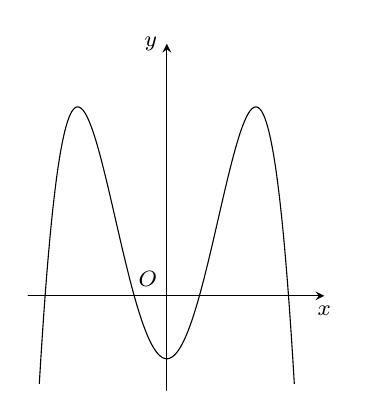
\begin{tikzpicture}[scale=0.8, font=\footnotesize, line join=round, line cap=round,>=stealth]
			\def\a{-1} \def\b{4} \def\c{-1} % Hệ số
			\def\xmin{-2.2} \def\xmax{2.5}
			\def\ymin{-1.5} \def\ymax{4} 
			\draw[->] (\xmin,0)--(\xmax,0) node [below]{$x$};
			\draw[->] (0,\ymin)--(0,\ymax) node [left]{$y$};
			\node at (0,0) [above left]{$O$};
			\clip (\xmin+0.1,\ymin+0.1) rectangle (\xmax-0.1,\ymax-0.1);
			\draw[smooth,samples=300] plot(\x,{\a*(\x)^4+\b*(\x)^2+\c});
		\end{tikzpicture}
	\end{center}
	Mệnh đề nào dưới đây đúng?
	\choice
	{\True $a<0$, $b>0$, $c<0$}
	{$a<0$, $b<0$, $c>0$}
	{$a<0$, $b>0$, $c>0$}
	{$a<0$, $b<0$, $c<0$}
	\loigiai{
		Đồ thị cắt trục tung tại điểm $(0;c)$, từ đồ thị suy ra $c<0$.\\
		Mặt khác đồ thị hàm số có ba điểm cực trị nên $y'=0$ có ba nghiệm phân biệt, hay $y'=4ax^3+2bx=2x\left(2ax^2+b\right)=0$ có ba nghiệm phân biệt. Suy ra $a,b$ trái dấu.\\
		Mà $a<0\Rightarrow b>0$.}
\end{ex}
\begin{ex}%Câu 17.%[2D1B5-1]
	[Cụm Liên Trường Hải Phòng 2019]
	Hàm số $y=ax^3+bx^2+cx+d$ có đồ thị như hình vẽ bên dưới: 
	\begin{center}
		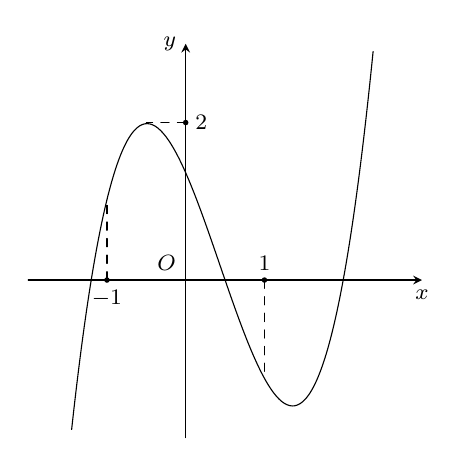
\begin{tikzpicture}[scale=1, font=\footnotesize, line join=round, line cap=round,>=stealth]
			\def\a{1.135}  % Hệ số co dãn
			\def\xmin{-2} \def\xmax{3}
			\def\ymin{-2} \def\ymax{3} 
			\draw[->] (\xmin,0)--(\xmax,0) node [below]{$x$};
			\draw[->] (0,\ymin)--(0,\ymax) node [left]{$y$};
			\node at (0,0) [above left]{$O$};
			\clip (\xmin+0.1,\ymin+0.1) rectangle (\xmax-0.1,\ymax-0.1);
			\draw[smooth,samples=300] plot(\x,{\a*((\x+1.2)*(\x-0.5)*(\x-2))});
			\draw[dashed] (-1,0)--(-1,1) (1,0)--(1,-1.2) (0,2)--(-0.5,2);
			\fill (-1,0) circle (1.0pt) node[below]{$-1$} 
			(1,0) circle (1.0pt) node[above]{$1$}
			(0,2) circle (1.0pt) node[right]{$2$};
		\end{tikzpicture}
	\end{center}
	Khẳng định nào là đúng?
	\choice
	{$a<0$, $b<0$, $c<0$, $d<0$}
	{$a>0$, $b>0$, $c>0$, $d<0$}
	{$a>0$, $b>0$, $c<0$, $d>0$}
	{\True $a>0$, $b<0$, $c<0$, $d>0$}
	\loigiai{
		+ Dựa vào hình dạng đồ thị ta khẳng định được $a>0$.\\
		+ Đồ thị cắt trục $Oy$ tại điểm có tọa độ $(0;d)$. Dựa vào đồ thị suy ra $d>0$.\\
		+ Ta có: $y'=3ax^2+2bx+c$. Hàm số có hai điểm cực trị $x_1$, $x_2 (x_1<x_2)$ trái dấu nên phương trình $y'=0$ có hai nghiệm phân biệt $x_1$, $x_2$ trái dấu. Vì thế $3a\cdot c<0$, nên suy ra $c<0$.\\
		+ Mặt khác từ đồ thị ta thấy $\heva{&x_1 >-1\\&x_2>1}$ nên $x_1+x_2>0$.\\
		Mà $x_1+x_2=\dfrac{-2b}{3a}$ nên suy ra $\dfrac{-2b}{3a}>0\Rightarrow b<0$.\\
		Vậy $a>0$, $b<0$, $c<0$, $d>0$.}
\end{ex}
\begin{ex}%Câu 18.%[2D1B5-1]
	[THPT Ba Đình 2019] Cho hàm số $y=\dfrac{ax+b}{x+c}$ có đồ thị như hình bên dưới, với $a$, $b$, $c\in\mathbb{Z}$. Tính giá trị của biểu thức $T=a+2b+3c$?
	\begin{center}
		\begin{tikzpicture}[scale=0.7, font=\footnotesize, line join=round, line cap=round,>=stealth]
			\def\a{-1} \def\b{2} \def\c{1} \def\d{-1} % Hệ số
			\def\xmin{-4} \def\xmax{5}
			\def\ymin{-4} \def\ymax{4.5}
			\draw[->] (\xmin,0)--(\xmax,0) node [below]{$x$};
			\draw[->] (0,\ymin)--(0,\ymax) node [left]{$y$};
			\node at (0,0) [above left]{$O$};
			\clip (\xmin+0.1,\ymin+0.1) rectangle (\xmax-0.1,\ymax-0.1);
			\draw[smooth,samples=300,domain=\xmin:(-\d/\c-0.1)] plot(\x,{(\a*(\x)+\b)/(\c*(\x)+\d)});
			\draw[smooth,samples=300,domain=(-\d/\c+0.1:\xmax)] plot(\x,{(\a*(\x)+\b)/(\c*(\x)+\d)});
			\draw[dashed] (-\d/\c,\ymin)--(-\d/\c,\ymax);
			\draw[dashed] (\xmin,\a/\c)--(\xmax,\a/\c);
			\fill (1,0) circle (1.0pt) node[above left]{$1$} (2,0) circle (1.0pt) node[below left]{$2$} (0,-1) circle (1.0pt) node[below left]{$-1$} (0,-2) circle (1.0pt) node[right]{$-2$};
		\end{tikzpicture}
	\end{center}
	\choice
	{$T=-8$}
	{$T=2$}
	{$T=6$}
	{\True $T=0$}
	\loigiai{
		Từ đồ thị hàm số, ta suy ra\\
		Đồ thị hàm số có tiệm cận đứng là đường thẳng $x=1$, tiệm cận ngang là đường thẳng $y=-1$.\\
		Đồ thị hàm số đi qua các điểm $A(2;0)$, $B(0;-2)$.\\
		Từ biểu thức hàm số $y=\dfrac{ax+b}{x+c}$ (vì đồ thị hàm số là đồ thị hàm nhất biến nên $ac-b\neq 0$), ta suy ra\\
		Đồ thị hàm số có tiệm cận đứng là đường thẳng $x=-c$, tiệm cận ngang là đường thẳng $y=a$.\\
		Đồ thị hàm số đi qua $A\left(-\dfrac{b}{a};0\right)$, $B\left(0;\dfrac{b}{c}\right)$.\\
		Đối chiếu lại, ta suy ra $c=-1$, $a=-1$, $b=2$.\\
		Vậy $T=a+2b+3c=(-1)+2\cdot 2+3(-1)=0$.}
\end{ex}
\begin{ex}%Câu 19.%[2D1B5-1]
	[THPT Việt Đức Hà Nội 2019]
	\immini
	{
		Cho hàm số $y=ax^3+bx^2+cx+d$ có đồ thị như hình bên. Trong các mệnh đề sau mệnh đề nào đúng?	
	\choice
	{\True $ab<0,bc>0,cd<0$}
	{$ab<0,bc<0,cd>0$}
	{$ab>0,bc>0,cd<0$}
	{$ab>0,bc>0,cd>0$}
	}
	{
		\begin{tikzpicture}[scale=1, font=\footnotesize, line join=round, line cap=round,>=stealth]
			\def\a{0.5}  % Hệ số co dãn
			\def\xmin{-1.3} \def\xmax{4}
			\def\ymin{-2.5} \def\ymax{2} 
			\draw[->] (\xmin,0)--(\xmax,0) node [below]{$x$};
			\draw[->] (0,\ymin)--(0,\ymax) node [left]{$y$};
			\node at (0,0) [below left]{$O$};
			\clip (\xmin+0.1,\ymin+0.1) rectangle (\xmax-0.1,\ymax-0.1);
			\draw[smooth,samples=300] plot(\x,{\a*((\x+0.8)*(\x-0.6)*(\x-3))});
		\end{tikzpicture}
	}
	\loigiai{
		Từ dáng điệu của đồ thị ta có ngay được:\\
		$\oplus\lim\limits_{x\to+\infty} y=+\infty;\lim\limits_{x\to-\infty} y=-\infty\Rightarrow a>0$.\\
		$\oplus$ Đồ thị hàm số cắt trục tung tại một điểm có tung độ dương nên $d>0$.\\
		Ta có: $y'=3ax^2+2bx+c$.\\
		Mặt khác dựa vào đồ thị ta thấy phương trình $y'=0$ có hai nghiệm trái dấu và tổng hai nghiệm này luôn dương nên $\heva{&ac<0\\&-\dfrac{2b}{3a}>}\Rightarrow\heva{&c<0\\&b<0}$ (do $a>0$).\\
		Do đó: $ab<0,bc>,cd<0$.}
\end{ex}
\begin{ex}%[2D1B5-1]%Câu 20.
	[THPT Lương Thế Vinh Hà Nội 2019]
	Cho hàm số $y=ax^3+bx^2+cx+d$ có đồ thị như hình dưới. Khẳng định nào sau đây đúng?
	\immini	{
		\choice
		{$a<0,b<0,c<0,d<0$}
		{$a<0,b>0,c>0,d>0$}
		{$a<0,b>0,c<0,d>0$}
		{\True $a<0,b>0,c>0,d<0$}
	}{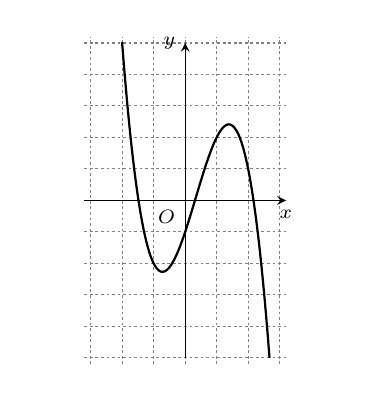
\begin{tikzpicture}[>=stealth,x=1cm,y=1cm,scale=0.4]
			\def\a{-1} % Hệ số a phải khác 0
			\def\b{1}
			\def\c{3}
			\def\d{-1}
			\draw[color=gray,dash pattern=on 1pt off 1pt,xstep=1.0cm,ystep=1.0cm] (-3.2,-5.2) grid (3.2,5.2);
			\draw[->] (-3.2,0) -- (3.2,0)node[below]{\scriptsize $x$};
			\draw[->] (0,-5) -- (0,5) node[left] {\scriptsize $y$};
			\draw (0,0)node[below left]{\scriptsize $O$};
			\clip (-5,-5)rectangle(5,5);
			\draw[thick,samples=150,smooth,domain=-5:5] plot(\x,{\a*(\x)^3+(\b)*(\x)^2+(\c)*\x+(\d)});
	\end{tikzpicture}}
	\loigiai{
		- Dựa vào hình dáng của đồ thị suy ra hệ số $a<0$.\\
		- Đồ thị cắt trục $Oy$ tại điểm có tung độ âm nên $d<0$.\\
		- Ta thấy đồ thị như hình vẽ có hai điểm cực trị, hoành độ các điểm cực trị trái dấu suy ra phương trình $y'=3ax^2+2bx+c=0$ có 2 nghiệm $x_1,x_2$ trái dấu kéo theo $3a\cdot c<0\Rightarrow c>0$.\\
		- Mặt khác $\dfrac{x_1+x_2}{2}=-\dfrac{b}{3a}>0\Rightarrow b>0$.}
\end{ex}
\begin{ex}%[2D1B5-1]%Câu 21.
	[THPT Chuyên Bắc Ninh 2019]
	\immini{Cho hàm số có đồ thị như hình vẽ. Mệnh đề nào dưới đây đúng?
		\choice
		{$a>0,b<0,c<0$}
		{$a<0,b<0,c<0$}
		{\True $a<0,b>0,c<0$}
		{$a>0,b<0,c>0$}} 	{% Đồ thị hàm y=ax^4+bx^2+c. Nếu hệ số lớn cần điều chỉnh hệ trục, vùng lưới, domain và lệnh \clip
		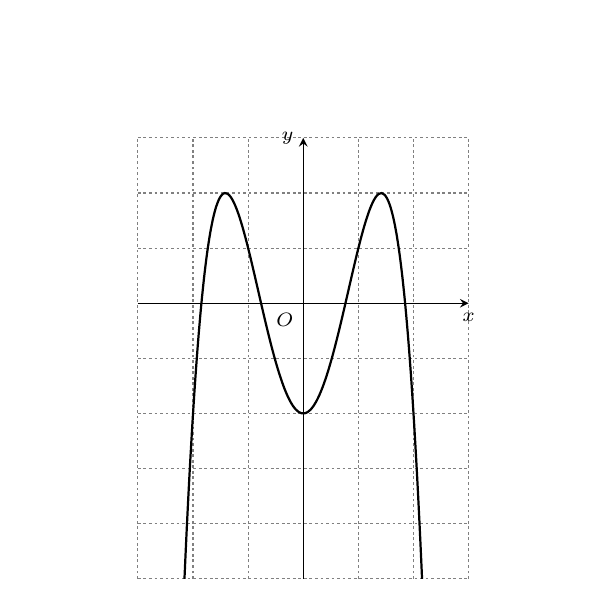
\begin{tikzpicture}[>=stealth,x=1cm,y=1cm,scale=0.7]
			\def\a{-1} % Hệ số a phải khác 0
			\def\b{4}
			\def\c{-2}
			\draw[color=gray,dash pattern=on 1pt off 1pt,xstep=1.0cm,ystep=1.0cm] (-3,-5) grid (3,3);
			\draw[->] (-3,0) -- (3,0) node[below] {\scriptsize $x$};
			\draw[->] (0,-5) -- (0,3) node[left] {\scriptsize $y$};
			\draw (0,0)node[below left]{\scriptsize $O$};
			\clip (-5,-5)rectangle(5,5);
			\draw[thick,samples=150,smooth,domain=-4:4] plot(\x,{\a*(\x)^4+(\b)*(\x)^2+(\c)});
		\end{tikzpicture}
	}
	\loigiai{
		- Dựa vào hình dạng đồ thị suy ra $a<0$.\\
		- Hàm số có 3 điểm cực trị nên $ab<0\Rightarrow b>0$.\\
		- Giao điểm với trục tung nằm dưới trục hoành nên $c<0$.}
\end{ex}
\begin{ex}%[2D1B5-1]%Câu 22.
	[Chuyên Lê Quý Đôn Quảng Trị 2019]
	\immini {Cho hàm số $y=\dfrac{ax+b}{cx+d}$ có đồ thị như trong hình bên dưới. Biết rằng $a$ là số thực dương, hỏi trong các số $b,c,d$ có tất cả bao nhiêu số dương?
		
		\choice
		{$1$}
		{\True $2$}
		{$0$}
		{$3$}
	}{
		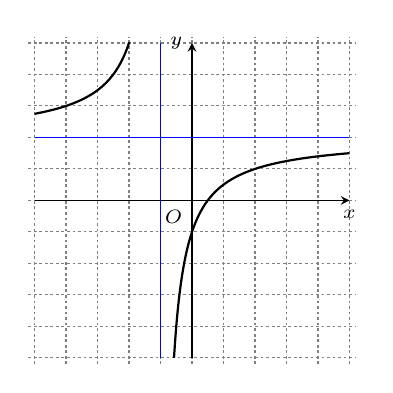
\begin{tikzpicture}[>=stealth,x=1cm,y=1cm,scale=0.4]
			\def\a{2}
			\def\b{-1}
			\def\c{1}
			\def\d{1}
			\draw[color=gray,dash pattern=on 1pt off 1pt,xstep=1.0cm,ystep=1.0cm] (-5.2,-5.2) grid (5.2,5.2);
			\draw[->] (-5,0) -- (5,0) node[below] {\scriptsize $x$};
			\draw[->] (0,-5) -- (0,5) node[left] {\scriptsize $y$};
			\draw (0,0)node[below left]{\scriptsize $O$};
			\draw[blue] (-1,-5)--(-1,5) (-5,2)--(5,2); % Vẽ TCĐ và TCN
			\clip (-5,-5)rectangle(5,5);
			\pgfmathsetmacro{\can}{-(\d)/(\c)}
			\draw[thick,samples=150,smooth,domain=-5:{\can-.1}] plot(\x,{(\a*\x+(\b))/(\c*\x+(\d))}); % Vẽ nhánh bên trái TCĐ
			\draw[thick,samples=150,smooth,domain={\can+.1}:5] plot(\x,{(\a*\x+(\b))/(\c*\x+(\d))}); % Vẽ nhánh bên phải TCĐ
		\end{tikzpicture}
	}
	\loigiai{
		Nhìn vào đồ thị ta thấy.\\
		tiệm cận ngang $y=\dfrac{a}{c}$ nằm trên trục hoành nên $c>0$ (vì $a>0$).\\
		tiệm cận đứng $x=\dfrac{-d}{c}$ nằm bên trái trục tung nên $\dfrac{-d}{c}<0$. Suy ra $d>0$ (vì $c>0$).\\
		giao điểm của đồ thị và trục tung nằm bên dưới trục hoành nên $\dfrac{b}{d}<0$.\\
		Suy ra $b<0$ (vì $d>0$).\\
		Vậy $c>0,d>0$.}
\end{ex}
\begin{ex}%[2D1B5-1]%Câu 23.
	[Cụm liên trường Hải Phòng 2019]
	\immini {Hàm số $y=ax^3+bx^2+cx+d$ có đồ thị như hình vẽ bên dưới. Khẳng định nào là đúng?
		\choice
		{$a<0$, $b<0$, $c<0$, $d<0$}
		{$a>0$, $b>0$, $c>0$, $d<0$}
		{$a>0$, $b>0$, $c<0$, $d>0$}
		{\True $a>0$, $b<0$, $c<0$, $d>0$}}
	{% Đồ thị hàm y=ax^3+bx^2+cx+d. Nếu hệ số lớn cần điều chỉnh hệ trục, vùng lưới, domain và lệnh \clip
		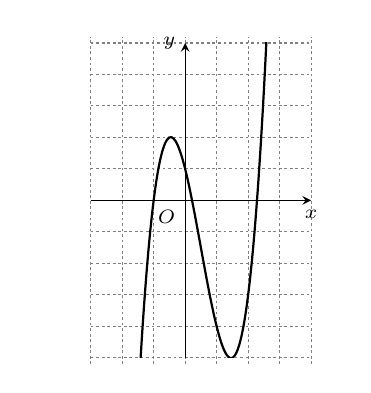
\begin{tikzpicture}[>=stealth,x=1cm,y=1cm,scale=0.4]
			\def\a{2} % Hệ số a phải khác 0
			\def\b{-3}
			\def\c{-4}
			\def\d{1}
			\draw[color=gray,dash pattern=on 1pt off 1pt,xstep=1.0cm,ystep=1.0cm] (-3,-5.2) grid (4,5.2);
			\draw[->] (-3,0) -- (4,0)node[below]{\scriptsize $x$};
			\draw[->] (0,-5) -- (0,5) node[left] {\scriptsize $y$};
			\draw (0,0)node[below left]{\scriptsize $O$};
			\clip (-5,-5)rectangle(5,5);
			\draw[thick,samples=150,smooth,domain=-5:5] plot(\x,{\a*(\x)^3+(\b)*(\x)^2+(\c)*\x+(\d)});
		\end{tikzpicture}
	}
	\loigiai{
		+ Dựa vào hình dạng đồ thị ta khẳng định được $a>0$.\\
		+ Đồ thị cắt trục $Oy$ tại điểm có tọa độ $(0;d)$. Dựa vào đồ thị suy ra $d>0$.\\
		+ Ta có: $y'=3ax^2+2bx+c$. Hàm số có hai điểm cực trị $x_1$, $x_2 (x_1<x_2)$ trái dấu nên phương trình $y'=0$ có hai nghiệm phân biệt $x_1$, $x_2$ trái dấu. Vì thế $3a\cdot c<0$, nên suy ra $c<0$.\\
		+ Mặt khác từ đồ thị ta thấy $\heva{&x_1 >-1\\&x_2>1}$ nên $x_1+x_2>0$.\\
		Mà $x_1+x_2=\dfrac{-2b}{3a}$ nên suy ra $\dfrac{-2b}{3a}>0\Rightarrow b<0$.\\
		Vậy $a>0$, $b<0$, $c<0$, $d>0$.}
\end{ex}
\begin{ex}%[2D1B5-1]%Câu 24.
	[Chuyên Nguyễn Huệ 2019]
	\immini{ Cho hàm số $y=\dfrac{ax+b}{cx+d}$ có đồ thị như hình vẽ bên. Khẳng định nào sau đây là khẳng định đúng?
		\choice
		{$\heva{&ad<0\\&bc>0}$}
		{$\heva{&ad<0\\&bc<0}$}
		{\True $\heva{&ad>0\\&bc<0}$}
		{$\heva{&ad>0\\&bc>0}$}}
	{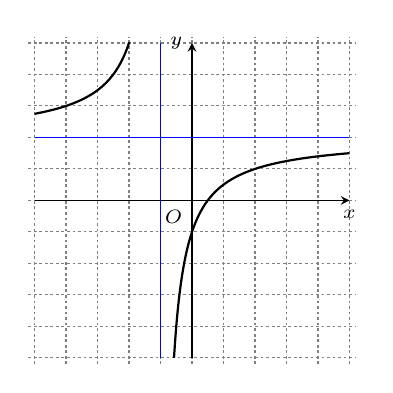
\begin{tikzpicture}[>=stealth,x=1cm,y=1cm,scale=0.4]
			\def\a{2}
			\def\b{-1}
			\def\c{1}
			\def\d{1}
			\draw[color=gray,dash pattern=on 1pt off 1pt,xstep=1.0cm,ystep=1.0cm] (-5.2,-5.2) grid (5.2,5.2);
			\draw[->] (-5,0) -- (5,0) node[below] {\scriptsize $x$};
			\draw[->] (0,-5) -- (0,5) node[left] {\scriptsize $y$};
			\draw (0,0)node[below left]{\scriptsize $O$};
			\draw[blue] (-1,-5)--(-1,5) (-5,2)--(5,2); % Vẽ TCĐ và TCN
			\clip (-5,-5)rectangle(5,5);
			\pgfmathsetmacro{\can}{-(\d)/(\c)}
			\draw[thick,samples=150,smooth,domain=-5:{\can-.1}] plot(\x,{(\a*\x+(\b))/(\c*\x+(\d))}); % Vẽ nhánh bên trái TCĐ
			\draw[thick,samples=150,smooth,domain={\can+.1}:5] plot(\x,{(\a*\x+(\b))/(\c*\x+(\d))}); % Vẽ nhánh bên phải TCĐ
	\end{tikzpicture}}
	\loigiai{
		Nhận xét từ đồ thị:\\
		+ Giao với trục hoành tại $x_o=-\dfrac{b}{a}>0\Rightarrow a$ và $b$ trái dấu (1).\\
		+ Giao với trục tung tại $y_o=\dfrac{b}{d}<0\Rightarrow b$ và $d$ trái dấu (2).\\
		+ Tiệm cận đứng: $x=-\dfrac{d}{c}<0\Rightarrow d$ và $c$ cùng dấu (3).\\
		Từ (1) và (2) suy ra: $a$ và $d$ cùng dấu hay $ad>0$.\\
		Từ (2) và (3) suy ra: $b$ và $c$ trái dấu hay $bc<0$.}
\end{ex}
\begin{ex}%[2D1B5-1]%Câu 25.
	Tìm đồ thị hàm số $y=f(x)$ được cho bởi một trong các phương án dưới đây, biết $f(x)=(a-x)(b-x)^2$ với $a<b$. 
	\choice
	{\True % Đồ thị hàm y=ax^3+bx^2+cx+d. Nếu hệ số lớn cần điều chỉnh hệ trục, vùng lưới, domain và lệnh \clip
		\begin{tikzpicture}[>=stealth,x=1cm,y=1cm,scale=0.4]
			\def\a{-1} % Hệ số a phải khác 0
			\def\b{7}
			\def\c{-15}
			\def\d{9}
			%	\draw[color=gray,dash pattern=on 1pt off 1pt,xstep=1.0cm,ystep=1.0cm] (-5.2,-5.2) grid (5.2,5.2);
			\draw[->] (-1,0) -- (5,0)node[below]{\scriptsize $x$};
			\draw[->] (0,-5) -- (0,5) node[left] {\scriptsize $y$};
			\draw (0,0)node[below left]{\scriptsize $O$};
			\clip (-5,-5)rectangle(5,5);
			\draw[thick,samples=150,smooth,domain=-5:5] plot(\x,{\a*(\x)^3+(\b)*(\x)^2+(\c)*\x+(\d)});
		\end{tikzpicture}
	}
	{	\begin{tikzpicture}[>=stealth,x=1cm,y=1cm,scale=0.4]
			\def\a{-1} % Hệ số a phải khác 0
			\def\b{5}
			\def\c{-7}
			\def\d{3}
			%	\draw[color=gray,dash pattern=on 1pt off 1pt,xstep=1.0cm,ystep=1.0cm] (-5.2,-5.2) grid (5.2,5.2);
			\draw[->] (-1,0) -- (5,0)node[below]{\scriptsize $x$};
			\draw[->] (0,-5) -- (0,5) node[left] {\scriptsize $y$};
			\draw (0,0)node[below left]{\scriptsize $O$};
			\clip (-5,-5)rectangle(5,5);
			\draw[thick,samples=150,smooth,domain=-5:5] plot(\x,{\a*(\x)^3+(\b)*(\x)^2+(\c)*\x+(\d)});
	\end{tikzpicture}}
	{\begin{tikzpicture}[>=stealth,x=1cm,y=1cm,scale=0.4]
			\def\a{1} % Hệ số a phải khác 0
			\def\b{-5}
			\def\c{7}
			\def\d{-3}
			%	\draw[color=gray,dash pattern=on 1pt off 1pt,xstep=1.0cm,ystep=1.0cm] (-5.2,-5.2) grid (5.2,5.2);
			\draw[->] (-1,0) -- (5,0)node[below]{\scriptsize $x$};
			\draw[->] (0,-5) -- (0,5) node[left] {\scriptsize $y$};
			\draw (0,0)node[below left]{\scriptsize $O$};
			\clip (-5,-5)rectangle(5,5);
			\draw[thick,samples=150,smooth,domain=-5:5] plot(\x,{\a*(\x)^3+(\b)*(\x)^2+(\c)*\x+(\d)});
	\end{tikzpicture}}
	{\begin{tikzpicture}[>=stealth,x=1cm,y=1cm,scale=0.4]
			\def\a{1} % Hệ số a phải khác 0
			\def\b{-7}
			\def\c{15}
			\def\d{-9}
			%	\draw[color=gray,dash pattern=on 1pt off 1pt,xstep=1.0cm,ystep=1.0cm] (-5.2,-5.2) grid (5.2,5.2);
			\draw[->] (-1,0) -- (5,0)node[below]{\scriptsize $x$};
			\draw[->] (0,-5) -- (0,5) node[left] {\scriptsize $y$};
			\draw (0,0)node[below left]{\scriptsize $O$};
			\clip (-5,-5)rectangle(5,5);
			\draw[thick,samples=150,smooth,domain=-5:5] plot(\x,{\a*(\x)^3+(\b)*(\x)^2+(\c)*\x+(\d)});
	\end{tikzpicture}}
	\loigiai{
		Có $f'(x)=-(b-x)^2+(a-x)\cdot (-2)(b-x)=-(b-x)(b-x+2a-2x)=-(b-x)(b+2a-3x)$.\\
		$f'(x)=0\Leftrightarrow\hoac{&x=b\\&x=\dfrac{2a+b}{3}.}$ \\
		Có $\dfrac{2a+b}{3}<\dfrac{2b+b}{3}=b$.\\
		Ta có bảng biến thiên
		\begin{center}
			% Cần khai báo \usepackage{tkz-tab}
			
\begin{tikzpicture}[>=stealth]
				\tkzTabInit[nocadre=false,lgt=1,espcl=2,deltacl=0.5]{$x$/.7 ,$y'$/.7,$y$/2}
				{$-\infty$ , $\frac{2a+b}{3}$ , $b$ , $+\infty$}
				\tkzTabLine{ , - , $0$ , + , $0$ , - , }
				\tkzTabVar{-/$-\infty$ , +/ , -/ , +/$+\infty$}
			\end{tikzpicture}
		\end{center}
	}
\end{ex}
\begin{ex}%[2D1B5-1]%Câu 26.
	\immini{Cho đường cong $(C)\colon y=ax^3+bx^2+cx+d$ có đồ thị như hình bên. 
		Khẳng định nào sau đây là đúng?
		\choice
		{$a>0, b<0, c<0, d<0$}
		{$a>0, b>0, c<0, d>0$}
		{$a<0, b>0, c>0, d<0$}
		{\True $a>0, b>0, c<0, d<0$}}
	{% Đồ thị hàm y=ax^3+bx^2+cx+d. Nếu hệ số lớn cần điều chỉnh hệ trục, vùng lưới, domain và lệnh \clip
		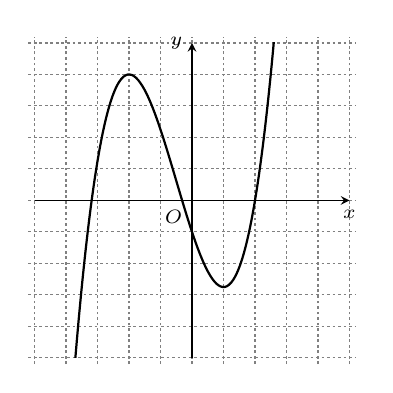
\begin{tikzpicture}[>=stealth,x=1cm,y=1cm,scale=0.4]
			\def\a{1/2} % Hệ số a phải khác 0
			\def\b{3/4}
			\def\c{-3}
			\def\d{-1}
			\draw[color=gray,dash pattern=on 1pt off 1pt,xstep=1.0cm,ystep=1.0cm] (-5.2,-5.2) grid (5.2,5.2);
			\draw[->] (-5,0) -- (5,0)node[below]{\scriptsize $x$};
			\draw[->] (0,-5) -- (0,5) node[left] {\scriptsize $y$};
			\draw (0,0)node[below left]{\scriptsize $O$};
			\clip (-5,-5)rectangle(5,5);
			\draw[thick,samples=150,smooth,domain=-5:5] plot(\x,{\a*(\x)^3+(\b)*(\x)^2+(\c)*\x+(\d)});
		\end{tikzpicture}
		
	}
	\loigiai{
		Từ đồ thị ta có $x=0\Rightarrow y=d<0$, từ dạng đồ thị suy ra $a>0$.\\
		Mặt khác $y'=3ax^2+2bx+c$ từ đồ thị ta có phương trình $y'=0$ có hai nghiệm trái dấu suy ra $ac<0$ mà $a>0$ suy ra $c<0$.\\
		Hơn nữa phương trình $y'=0$ có hai nghiệm phân biệt $x_1+x_2=-\dfrac{2b}{3a}=-1$ suy ra $3a=2b\Rightarrow b>0$.
	}
\end{ex}
\begin{ex}%[2D1B5-1]%Câu 27.
	[Gia Lai 2019] 
	\immini {Hàm số $y=ax^4+bx^2+c$ có đồ thị như hình vẽ bên. Mệnh đề nào sau đây đúng?
		
		\choice
		{$a>0$, $b>0$, $c<0$}
		{$a<0$, $b>0$, $c<0$}
		{\True $a>0$, $b<0$, $c>0$}
		{$a>0$, $b<0$, $c<0$}}
	{% Đồ thị hàm y=ax^4+bx^2+c. Nếu hệ số lớn cần điều chỉnh hệ trục, vùng lưới, domain và lệnh \clip
		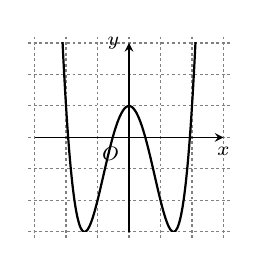
\begin{tikzpicture}[>=stealth,x=1cm,y=1cm,scale=0.4]
			\def\a{1} % Hệ số a phải khác 0
			\def\b{-4}
			\def\c{1}
			\draw[color=gray,dash pattern=on 1pt off 1pt,xstep=1.0cm,ystep=1.0cm] (-3.2,-3.2) grid (3.2,3.2);
			\draw[->] (-3,0) -- (3,0) node[below] {\scriptsize $x$};
			\draw[->] (0,-3) -- (0,3) node[left] {\scriptsize $y$};
			\draw (0,0)node[below left]{\scriptsize $O$};
			\clip (-3,-3)rectangle(3,3);
			\draw[thick,samples=150,smooth,domain=-4:4] plot(\x,{\a*(\x)^4+(\b)*(\x)^2+(\c)});
		\end{tikzpicture}
	}
	\loigiai{
		Dựa vào đồ thị:\\
		+ $\lim\limits_{x\to+\infty} y=+\infty\Rightarrow a>0$.\\
		+ Đồ thị hàm số có ba điểm cực trị $\Rightarrow ab<0\Rightarrow b<0$.\\
		+ Giao điểm của đồ thị hàm số và trục tung có tung độ dương $\Rightarrow$.\\
		Vậy $a>0$, $b<0$, $c>0$.}
\end{ex}
\begin{ex}%[2D1B5-1]%Câu 28.
	[THPT Thăng Long 2019] 
	\immini {Cho hàm số $y=ax^4+bx^2+c$ có đồ thị như hình vẽ. Tìm kết luận đúng
		\choice
		{$a+b>0$}
		{\True $bc>0$}
		{$ab>0$}
		{$ac>0$}}
	{% Đồ thị hàm y=ax^4+bx^2+c. Nếu hệ số lớn cần điều chỉnh hệ trục, vùng lưới, domain và lệnh \clip
		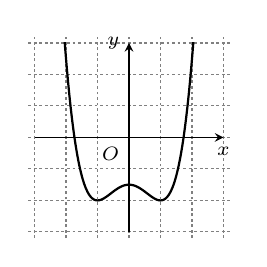
\begin{tikzpicture}[>=stealth,x=1cm,y=1cm,scale=0.4]
			\def\a{1/2} % Hệ số a phải khác 0
			\def\b{-1}
			\def\c{-3/2}
			\draw[color=gray,dash pattern=on 1pt off 1pt,xstep=1.0cm,ystep=1.0cm] (-3.2,-3.2) grid (3.2,3.2);
			\draw[->] (-3,0) -- (3,0) node[below] {\scriptsize $x$};
			\draw[->] (0,-3) -- (0,3) node[left] {\scriptsize $y$};
			\draw (0,0)node[below left]{\scriptsize $O$};
			\clip (-3,-3)rectangle(3,3);
			\draw[thick,samples=150,smooth,domain=-4:4] plot(\x,{\a*(\x)^4+(\b)*(\x)^2+(\c)});
		\end{tikzpicture}
	}
	\loigiai{
		Từ hình vẽ ta thấy:\\
		Đồ thị hàm số có bề lõm hướng lên $\Rightarrow a>0$.\\
		Đồ thị hàm số cắt trục tung tại điểm có tung độ âm $\Rightarrow c<0$.\\
		Đồ thị hàm số có 3 điểm cực trị $\Rightarrow ab<0\Rightarrow b<0$.\\
		Vậy chỉ có $bc>0$.}
\end{ex}
\begin{ex}%[2D1B5-1]%Câu 29.
	[THPT Cẩm Bình Hà Tĩnh 2019]
	\immini {Cho hàm số $y=ax^4+bx^2+c (a\neq 0)$ có đồ thị như hình bên. Hãy chọn mệnh đề đúng. 
		\choice
		{$a<0, b<0, c=0$}
		{$a<0, b>0, c=0$}
		{\True $a>0, b<0, c=0$}
		{$a>0, b<0, c>0$}}
	{% Đồ thị hàm y=ax^4+bx^2+c. Nếu hệ số lớn cần điều chỉnh hệ trục, vùng lưới, domain và lệnh \clip
		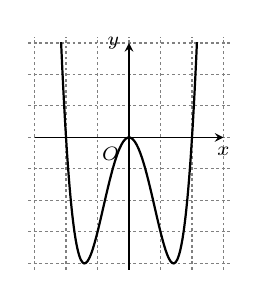
\begin{tikzpicture}[>=stealth,x=1cm,y=1cm,scale=0.4]
			\def\a{1} % Hệ số a phải khác 0
			\def\b{-4}
			\def\c{0}
			\draw[color=gray,dash pattern=on 1pt off 1pt,xstep=1.0cm,ystep=1.0cm] (-3.2,-4.2) grid (3.2,3.2);
			\draw[->] (-3,0) -- (3,0) node[below] {\scriptsize $x$};
			\draw[->] (0,-4.2) -- (0,3) node[left] {\scriptsize $y$};
			\draw (0,0)node[below left]{\scriptsize $O$};
			\clip (-3,-4.2)rectangle(3,3);
			\draw[thick,samples=150,smooth,domain=-4:4] plot(\x,{\a*(\x)^4+(\b)*(\x)^2+(\c)});
		\end{tikzpicture}
	}
	\loigiai{
		Dựa vào hình dạng đồ thị hàm số ta nhận thấy:\\
		Hệ số $a>0$.\\
		Đồ thị hàm số đi qua gốc tọa tọa $\Rightarrow c=0$.\\
		Hàm số có 3 điểm cực trị $\Rightarrow a\cdot b<0\Rightarrow b<0$.}
\end{ex}
\begin{ex}%[2D1B5-1]%Câu 30.
	[Chuyên Long An 2019]
	\immini {Cho hàm số $y=f(x)=ax^3+bx^2+cx+d$ có đồ thị như hình vẽ ở bên. Mệnh đề nào
		sau đây đúng?		
		\choice
		{$a>0$, $b>0$, $c>0$, $d>0$}
		{$a>0$, $b>0$, $c<0$, $d>0$}
		{\True $a>0$, $b<0$, $c>0$, $d>0$}
		{$a<0$, $b<0$, $c>0$, $d<0$}}
	{
		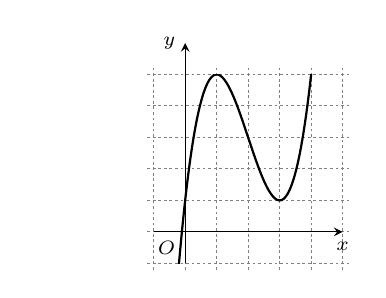
\begin{tikzpicture}[>=stealth,x=1cm,y=1cm,scale=0.4]
			\def\a{1} % Hệ số a phải khác 0
			\def\b{-6}
			\def\c{9}
			\def\d{1}
			\draw[color=gray,dash pattern=on 1pt off 1pt,xstep=1.0cm,ystep=1.0cm] (-1.2,-1.2) grid (5.2,5.2);
			\draw[->] (-1,0) -- (5,0)node[below]{\scriptsize $x$};
			\draw[->] (0,-1) -- (0,6) node[left] {\scriptsize $y$};
			\draw (0,0)node[below left]{\scriptsize $O$};
			\clip (-5,-1)rectangle(5,5);
			\draw[thick,samples=150,smooth,domain=-5:5] plot(\x,{\a*(\x)^3+(\b)*(\x)^2+(\c)*\x+(\d)});
		\end{tikzpicture}
	}
	\loigiai{
		Đồ thị hàm số đi qua các điểm $A(0;1)$, $B(1;5)$ và $C(3;1)$ và đạt cực trị tại các điểm $B$ và $C$.\\
		$f'(x)=3ax^2+2bx+c$. Ta có\\
		$\heva{&f(0)=1\\&f(1)=5\\&f'(1)=0\\&f'(3)=0}\Rightarrow\heva{&d=1\\&a+b+c+d=5\\&3a+2b+c=0\\&27a+6b+c=0}\Rightarrow\heva{&a=1\\&b=-6\\&c=9\\&d=1}$.}
\end{ex}
\begin{ex}%[2D1B5-1]%Câu 31.
	[THPT Trần Phú 2019] 
	\immini{Cho hàm số bậc bốn trùng phương $y=ax^4+bx^2+c$ có đồ thị như hình vẽ bên. Mệnh đề nào dưới đây là đúng?
		\choice
		{$a<0, b>0, c>0$}
		{$a>0, b<0, c>0$}
		{\True $a<0, b>0, c=0$}
		{$a>0, b<0, c<0$}}
	{% Đồ thị hàm y=ax^4+bx^2+c. Nếu hệ số lớn cần điều chỉnh hệ trục, vùng lưới, domain và lệnh \clip
		\begin{tikzpicture}[>=stealth,x=1cm,y=1cm,scale=0.7]
			\def\a{1} % Hệ số a phải khác 0
			\def\b{-4}
			\def\c{4}
			\draw[color=gray,dash pattern=on 1pt off 1pt,xstep=1.0cm,ystep=1.0cm] (-3.2,-1.2) grid (3.2,5.2);
			\draw[->] (-3,0) -- (3,0) node[below] {\scriptsize $x$};
			\draw[->] (0,-1) -- (0,5) node[left] {\scriptsize $y$};
			\draw (0,0)node[below left]{\scriptsize $O$};
			\clip (-5,-5)rectangle(5,5);
			\draw[thick,samples=150,smooth,domain=-4:4] plot(\x,{\a*(\x)^4+(\b)*(\x)^2+(\c)});
		\end{tikzpicture}
	}
	\loigiai{
		Dựa vào hình dạng đồ thị hàm số ta nhận thấy:\\
		Hệ số $a<0$.\\
		Hàm số có 3 điểm cực trị $\Rightarrow a\cdot b<0\Rightarrow b>0$.\\
		Đồ thị hàm số đi qua gốc tọa độ $\Rightarrow c=0$.\\
		Vậy $a<0, b>0, c=0$.}
\end{ex}
\begin{ex}%[2D1B5-1]%Câu 32.
	[THPT Cộng Hiền 2019] 
	\immini {Cho hàm số $y=ax^4+bx^2+c$ có đồ thị như hình vẽ bên. Hỏi khẳng định nào sau đây đúng?
		\choice
		{\True $a>0, b<0, c<0$}
		{$a>0, b>0, c<0$}
		{$a>0, b<0, c>0$}
		{$a<0, b>0, c<0$}}
	{ % Đồ thị hàm y=ax^4+bx^2+c. Nếu hệ số lớn cần điều chỉnh hệ trục, vùng lưới, domain và lệnh \clip
		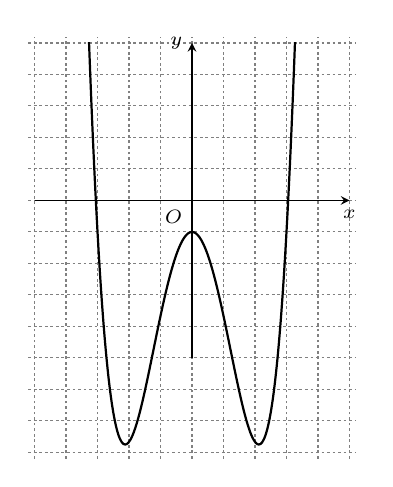
\begin{tikzpicture}[>=stealth,x=1cm,y=1cm,scale=0.4]
			\def\a{1/3} % Hệ số a phải khác 0
			\def\b{-3}
			\def\c{-1}
			\draw[color=gray,dash pattern=on 1pt off 1pt,xstep=1.0cm,ystep=1.0cm] (-5.2,-8.2) grid (5.2,5.2);
			\draw[->] (-5,0) -- (5,0) node[below] {\scriptsize $x$};
			\draw[->] (0,-5) -- (0,5) node[left] {\scriptsize $y$};
			\draw (0,0)node[below left]{\scriptsize $O$};
			\clip (-5,-8)rectangle(5,5);
			\draw[thick,samples=150,smooth,domain=-4:4] plot(\x,{\a*(\x)^4+(\b)*(\x)^2+(\c)});
		\end{tikzpicture}
	}
	\loigiai{
		Nhìn vào đồ thị ta có:\\
		Khi $x\in (2;+\infty)$ hàm số đồng biến $\Rightarrow a>0$.\\
		Hàm số có $3$ điểm cực trị nên $a.b<0$ mà $a>0\Rightarrow b<0$.\\
		$y(0)=-1=c\Rightarrow c<0$.}
\end{ex}
\begin{ex}%[2D1B5-1]%Câu 33.
	[SGD Điện Biên - 2019] 
	\immini { Cho hàm số $y=\dfrac{ax+3}{x+c}$ có đồ thị như hình vẽ bên. Tính giá trị của $a-2c$. 
		\choice
		{\True $a-2c=3$}
		{$a-2c=-3$}
		{$a-2c=-1$}
		{$a-2c=-2$}}
	{% Đồ thị hàm y=(ax+b)/(cx+d), ad-bc khác 0. Nếu hệ số lớn cần điều chỉnh hệ trục, vùng lưới, domain và lệnh \clip
		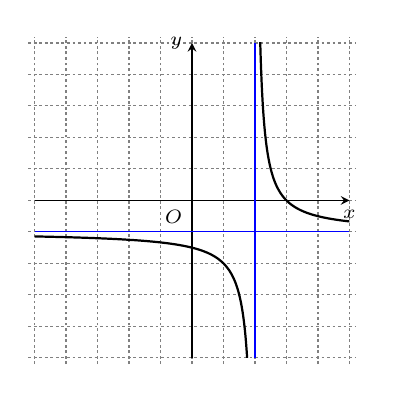
\begin{tikzpicture}[>=stealth,x=1cm,y=1cm,scale=0.4]
			\def\a{-1}
			\def\b{3}
			\def\c{1}
			\def\d{-2}
			\draw[color=gray,dash pattern=on 1pt off 1pt,xstep=1.0cm,ystep=1.0cm] (-5.2,-5.2) grid (5.2,5.2);
			\draw[->] (-5,0) -- (5,0) node[below] {\scriptsize $x$};
			\draw[->] (0,-5) -- (0,5) node[left] {\scriptsize $y$};
			\draw (0,0)node[below left]{\scriptsize $O$};
			\draw[blue] (2,-5)--(2,5) (-5,-1)--(5,-1); % Vẽ TCĐ và TCN
			\clip (-5,-5)rectangle(5,5);
			\pgfmathsetmacro{\can}{-(\d)/(\c)}
			\draw[thick,samples=150,smooth,domain=-5:{\can-.1}] plot(\x,{(\a*\x+(\b))/(\c*\x+(\d))}); % Vẽ nhánh bên trái TCĐ
			\draw[thick,samples=150,smooth,domain={\can+.1}:5] plot(\x,{(\a*\x+(\b))/(\c*\x+(\d))}); % Vẽ nhánh bên phải TCĐ
		\end{tikzpicture}
	}
	\loigiai{
		Đồ thị hàm số có TCN $y=-1\Leftrightarrow\dfrac{a}{1}=-1\Leftrightarrow a=-1$.\\
		Mặt khác Đồ thị hàm số có TCĐ $x=2$ nên $2+c=0\Leftrightarrow c=-2$ \\
		$\Rightarrow a-2c=-1-2\cdot (-2)=3$.\\
		Dựa vào đồ thị ta thấy các điểm $(3; 0)$ và $\left(0;-\dfrac{3}{2}\right)$ thuộc vào đồ thị hàm số đã cho nên ta được hệ phương trình $\heva{&0=\dfrac{a\cdot 3+3}{3+c}\\&-\dfrac{3}{2}=\dfrac{a\cdot 0+3}{0+c}}\Leftrightarrow\heva{&3a+3=0\\&-3c=6}\Leftrightarrow\heva{&a=-1\\&c=-2}$ \\
		$ \Rightarrow a-2c=-1-2\cdot (-2)=3 $.}
\end{ex}
\begin{ex}%[2D1B5-1]%Câu 34.
	\immini{Hình vẽ bên là đồ thị hàm số $y=\dfrac{ax+b}{cx+d}$. 
		Mệnh đề nào dưới đây đúng?
		\choice
		{$ad>0$ và $bd>0$}
		{\True $ad>0$ và $ab<0$}
		{$bd<0$ và $ab>0$}
		{$ad<0$ và $ab<0$}}
	{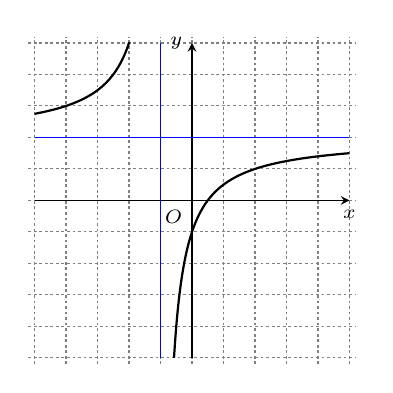
\begin{tikzpicture}[>=stealth,x=1cm,y=1cm,scale=0.4]
			\def\a{2}
			\def\b{-1}
			\def\c{1}
			\def\d{1}
			\draw[color=gray,dash pattern=on 1pt off 1pt,xstep=1.0cm,ystep=1.0cm] (-5.2,-5.2) grid (5.2,5.2);
			\draw[->] (-5,0) -- (5,0) node[below] {\scriptsize $x$};
			\draw[->] (0,-5) -- (0,5) node[left] {\scriptsize $y$};
			\draw (0,0)node[below left]{\scriptsize $O$};
			\draw[blue] (-1,-5)--(-1,5) (-5,2)--(5,2); % Vẽ TCĐ và TCN
			\clip (-5,-5)rectangle(5,5);
			\pgfmathsetmacro{\can}{-(\d)/(\c)}
			\draw[thick,samples=150,smooth,domain=-5:{\can-.1}] plot(\x,{(\a*\x+(\b))/(\c*\x+(\d))}); % Vẽ nhánh bên trái TCĐ
			\draw[thick,samples=150,smooth,domain={\can+.1}:5] plot(\x,{(\a*\x+(\b))/(\c*\x+(\d))}); % Vẽ nhánh bên phải TCĐ
	\end{tikzpicture}}
	\loigiai{
		Đồ thị hàm số giao với trục $Ox$ tại điểm có hoành độ $x=-\dfrac{b}{a}$, giao với $Oy$ tại điểm có tung độ $y=\dfrac{b}{d}$.\\
		Dựa vào hình vẽ ta có $\heva{&-\dfrac{b}{a}>0\\&\dfrac{b}{d}<0}\Leftrightarrow\heva{&\dfrac{b}{a}<0\\&\dfrac{b}{d}<0}\Leftrightarrow\heva{&ab<0\\&bd<0}\Rightarrow ad>0$.\\
		Trong các phương án chỉ có phương án B thỏa mãn.}
\end{ex}
\begin{ex}%[2D1B5-1]%Câu 35.
	\immini {Cho hàm số $y=\dfrac{ax-b}{x-1}$ có đồ thị như hình vẽ dưới đây: 
		Khẳng định nào sau đây đúng?
		\choice
		{\True $b<a<0$}
		{$a<b<0$}
		{$b>a$ và $a<0$}
		{$a<0<b$}}
	{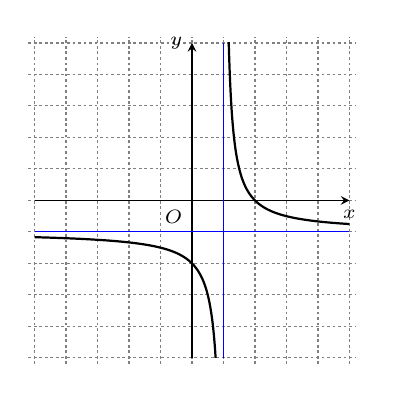
\begin{tikzpicture}[>=stealth,x=1cm,y=1cm,scale=0.4]
			\def\a{-1}
			\def\b{+2}
			\def\c{1}
			\def\d{-1}
			\draw[color=gray,dash pattern=on 1pt off 1pt,xstep=1.0cm,ystep=1.0cm] (-5.2,-5.2) grid (5.2,5.2);
			\draw[->] (-5,0) -- (5,0) node[below] {\scriptsize $x$};
			\draw[->] (0,-5) -- (0,5) node[left] {\scriptsize $y$};
			\draw (0,0)node[below left]{\scriptsize $O$};
			\draw[blue] (1,-5)--(1,5) (-5,-1)--(5,-1); % Vẽ TCĐ và TCN
			\clip (-5,-5)rectangle(5,5);
			\pgfmathsetmacro{\can}{-(\d)/(\c)}
			\draw[thick,samples=150,smooth,domain=-5:{\can-.1}] plot(\x,{(\a*\x+(\b))/(\c*\x+(\d))}); % Vẽ nhánh bên trái TCĐ
			\draw[thick,samples=150,smooth,domain={\can+.1}:5] plot(\x,{(\a*\x+(\b))/(\c*\x+(\d))}); % Vẽ nhánh bên phải TCĐ
	\end{tikzpicture}}
	\loigiai{
		Ta thấy đồ thị hàm số có tiệm cận ngang $y=-1$ suy ra $a=-1$.\\
		Do đồ thị hàm số đi qua điểm $(2;0)$ nên $2a-b=0\Leftrightarrow-2-b=0\Leftrightarrow b=-2$.\\
		Vậy $b<a<0$.}
\end{ex}
\begin{ex}%[2D1B5-1]%Câu 36.
	[Chuyên Lương Văn Chánh - Phú Yên - 2020] 
	\immini {Đồ thị trong hình bên dưới là của hàm số $y=\dfrac{ax+b}{x+c}$ (với $a,b,c\in\mathbb{R}$). 
		Khi đó tổng $a+b+c$ bằng
		\choice
		{$-1$}
		{$1$}
		{$2$}
		{\True $0$}}
	{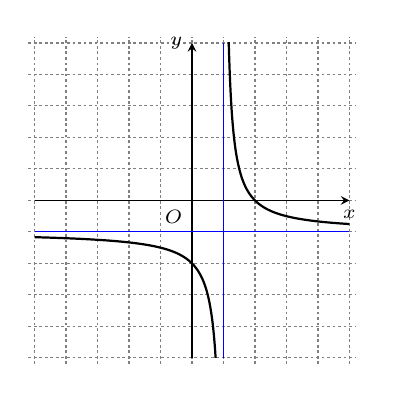
\begin{tikzpicture}[>=stealth,x=1cm,y=1cm,scale=0.4]
			\def\a{-1}
			\def\b{+2}
			\def\c{1}
			\def\d{-1}
			\draw[color=gray,dash pattern=on 1pt off 1pt,xstep=1.0cm,ystep=1.0cm] (-5.2,-5.2) grid (5.2,5.2);
			\draw[->] (-5,0) -- (5,0) node[below] {\scriptsize $x$};
			\draw[->] (0,-5) -- (0,5) node[left] {\scriptsize $y$};
			\draw (0,0)node[below left]{\scriptsize $O$};
			\draw[blue] (1,-5)--(1,5) (-5,-1)--(5,-1); % Vẽ TCĐ và TCN
			\clip (-5,-5)rectangle(5,5);
			\pgfmathsetmacro{\can}{-(\d)/(\c)}
			\draw[thick,samples=150,smooth,domain=-5:{\can-.1}] plot(\x,{(\a*\x+(\b))/(\c*\x+(\d))}); % Vẽ nhánh bên trái TCĐ
			\draw[thick,samples=150,smooth,domain={\can+.1}:5] plot(\x,{(\a*\x+(\b))/(\c*\x+(\d))}); % Vẽ nhánh bên phải TCĐ
	\end{tikzpicture}}
	\loigiai{
		Đồ thị hàm số $y=\dfrac{ax+b}{x+c}$ có đường tiệm cận ngang $y=a$, đường tiệm cận đứng $x=-c$ và cắt $Oy$ tại điểm $\left(0;\dfrac{b}{c}\right)$.\\
		Từ đồ thị hàm số ta có đường tiệm cận ngang $y=-1$, đường tiệm cận đứng $x=1$ và cắt $Oy$ tại điểm $(0;-2)$.\\
		Từ đó suy ra: $\heva{&a=-1\\&-c=1\\&\dfrac{b}{c}=-2}\Leftrightarrow\heva{&a=-1\\&c=-1\\&b=-2c}\Leftrightarrow\heva{&a=-1\\&c=-1\\&b=2}$. Vậy $a+b+c=-1-1+2=0$.}
\end{ex}
\begin{ex}%[2D1B5-1]%Câu 37.
	[Chuyên Lương Văn Tụy - Ninh Bình - 2020]
	\immini {Cho hàm số $f(x)=\dfrac{2-ax}{bx-c}\left(a,b,c\in\mathbb{R},b\neq 0\right)$ có bảng biến thiên như sau. Tổng các số $(a+b+c)^2$ thuộc khoảng nào sau đây
		\choice
		{$(1;2)$}
		{$(2;3)$}
		{\True $\left(0;\dfrac{4}{9}\right)$}
		{$\left(\dfrac{4}{9};1\right)$}
	}{
\begin{tikzpicture}[>=stealth]
			\tkzTabInit[nocadre=false,lgt=1,espcl=2,deltacl=0.5]{$x$/.7 ,$y'$/.7,$y$/2}
			{$-\infty$ , $1$ , $+\infty$}
			\tkzTabLine{ , + , d , + , }
			\tkzTabVar{-/$3$ ,+D-/$+\infty$/$-\infty$ , +/$3$}
		\end{tikzpicture}
	}
	\loigiai{
		Ta có $\lim\limits_{x\to\infty}\dfrac{2-ax}{bx-c}=\dfrac{-a}{b}$, theo giả thiết suy ra $\dfrac{-a}{b}=3\Leftrightarrow a=-3b$.\\
		Hàm số không xác định tại $x=1\Rightarrow b-c=0\Leftrightarrow b=c$.\\
		Hàm số đồng biến trên từng khoảng xác định nên $f'(x)=\dfrac{ac-2b}{(bx-c)^2}>0$ với mọi $x$ khác 1.
		Suy ra $ac-2b>0\Leftrightarrow-3b^2-2b>0\Leftrightarrow-\dfrac{2}{3}<b<0\Leftrightarrow 0 <-b<\dfrac{2}{3}$.\\
		Lại có $a+b+c=-3b+b+b=-b$. Suy ra $(a+b+c)^2=b^2\in\left(0;\dfrac{4}{9}\right)$.\\
		Vậy tổng $a+b+c$ thuộc khoảng $\left(0;\dfrac{4}{9}\right)$.}
\end{ex}
\begin{ex}%[2D1B5-1]%Câu 38.
	[Chuyên Hùng Vương - Gia Lai - 2020] 
	Cho hàm số $f(x)=\dfrac{ax+b}{cx+d} (a,b,c,d\in\mathbb{R}$ và $c\neq 0$). Biết rằng đồ thị hàm số đã cho đi qua điểm $(-1; 7)$ và giao điểm hai tiệm cận là $(-2; 3)$. Giá trị biểu thức $\dfrac{2a+3b+4c+d}{7c}$ bằng
	\choice
	{$7$}
	{$4$}
	{\True $6$}
	{$-5$}
	\loigiai{
		+ Ta có đồ thị hàm số $f(x)=\dfrac{ax+b}{cx+d}$ có đường tiệm cận ngang là $y=\dfrac{a}{c}$, đường tiệm cận đứng là $x=\dfrac{-d}{c}$.\\
		Theo bài ra, ta có: $\heva{&\dfrac{a}{c}=3\\&\dfrac{-d}{c}=-2}\Rightarrow\heva{&a=3c\\&d=2c.}$ \\
		+ Điểm $(-1; 7)$ thuộc đồ thị hàm số $f(x)$ nên $\dfrac{-a+b}{-c+d}=7\Leftrightarrow\dfrac{-3c+b}{-c+2c}=7\Leftrightarrow b=10c$.\\
		Vậy $\dfrac{2a+3b+4c+d}{7c}=\dfrac{2\cdot (3c)+3\cdot (10c)+4c+2c}{7c}=6$.}
\end{ex}
\begin{ex}%Câu 39.%[2D1B5-1]
	[Chuyên Lê Hồng Phong - Nam Định - 2020] Cho hàm số $y=\dfrac{ax+1}{bx+c}$ ($a$, $b$, $c$ là các tham số) có bảng biến thiên như hình vẽ
	\begin{center}
		
\begin{tikzpicture}
			\tkzTabInit[nocadre=false,lgt=1.2,espcl=3.5]
			{$ x $ /0.7, $ y' $ /0.7, $ y $ /2}
			{$ -\infty $, $ 2 $,  $ +\infty $}
			\tkzTabLine{,+, d,+, }
			\tkzTabVar{-/$1$,+D-/$+\infty$/$-\infty$,+/ $1$}
		\end{tikzpicture}
	\end{center}
	Xét các phát biểu sau: $(1)\colon c>1;$ \quad $(2)\colon a+b<0;$ \quad $(3)\colon a+b+c=0;$ \quad $(4)\colon a>0.$ Số phát biểu đúng là
	\choice
	{$1$}
	{\True $2$}
	{$3$}
	{$4$}
	\loigiai{
		Dựa vào bảng biến thiên ta có hàm số luôn đồng biến trên từng khoảng xác định, đồ thị hàm số có tiệm cận đứng là đường thẳng $x=2$ và tiệm cận ngang là đường thẳng $y=1$ nên ta có hệ.
		$$\heva{&-\dfrac{c}{b}=2\\&\dfrac{a}{b}=1\\&ac-b>0}\Leftrightarrow\heva{&c=-2b\\&a=b\\&ac-b>0}\Leftrightarrow\heva{&c=-2b\\&a=b\\&-2b^2-b>0}\Leftrightarrow\heva{&0<c<1\\&-\dfrac{1}{2}<a<0\\&-\dfrac{1}{2}<b<0\\&a+b+c=0.}$$
		Dựa vào hệ trên ta có các phát biểu $(1)$, $(4)$ là sai, $(2)$, $(3)$ đúng.}
\end{ex}
\begin{ex}%Câu 40.%[2D1B5-1]
	[Đô Lương 4 - Nghệ An - 2020] Ta xác định được các số $a$, $b$, $c$ để đồ thị hàm số $y=x^3+ax^2+bx+c$ đi qua điểm $(1;0)$ và có điểm cực trị $(-2;0)$. Tính giá trị biểu thức $T=a^2+b^2+c^2$. 
	\choice
	{\True $25$}
	{$-1$}
	{$7$}
	{$14$}
	\loigiai{
		Ta có $y=x^3+ax^2+bx+c\Rightarrow y'=3x^2+2ax+b$.\\
		Theo đề, ta có hệ phương trình $$\heva{&y(1)=0\\&y(-2)=0\\&y'(-2)=0}\Leftrightarrow\heva{&0=1^3+a{\cdot 1}^2+b\cdot 1+c\\&0=(-2)^3+a\cdot (-2)^2+b\cdot (-2)+c\\&0=3\cdot (-2)^2+2a\cdot (-2)+b} \Leftrightarrow\heva{&a+b+c=-1\\&4a-2b+c=8\\&-4a+b=-12}\Leftrightarrow\heva{&a=3\\&b=0\\&c=-4.} $$
		Vậy $T=a^2+b^2+c^2=3^2+0^2+(-4)^2=25$.}
\end{ex}
\begin{ex}%Câu 41.%[2D1B5-1]
	[Lê Lai - Thanh Hóa - 2020] Cho hàm số $y=ax^3+bx^2+cx+d$ có đồ thị như hình vẽ. Tính $S=a+b$?
	\begin{center}
		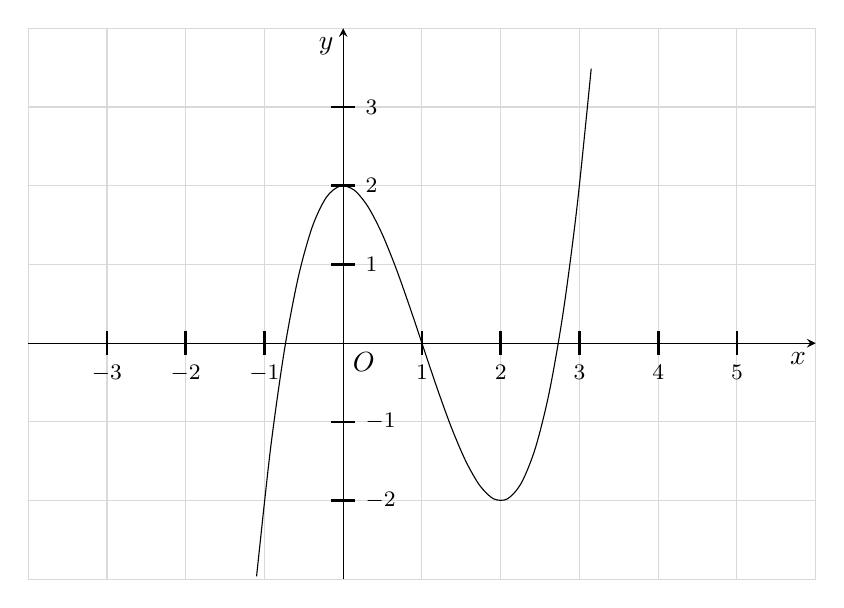
\begin{tikzpicture}[scale=1]
			\draw[step=1,gray!30,thin] (-4,-3) grid (6,4);
			\foreach \x in {-3,-2,-1,1,2,...,5}
			\draw[line width=1pt] (\x,-0.15) node[below]{ \footnotesize $\x$}--(\x,0.15) ;
			\foreach \y in {-2,-1,1,2,3}
			\draw[line width=1pt] (-0.15,\y)--(0.15,\y) node[right]{ \footnotesize $\y$} ;
			\draw[-stealth] (-4,0)--(6,0)node[below left]{$x$};
			\draw[-stealth] (0,-3)--(0,4)node[below left]{$y$};
			\draw[smooth] plot[domain=-1.1:3.15] (\x,{(\x)^3-3*(\x)^2+2}) (0,0) node[below right]{$O$};
		\end{tikzpicture}
	\end{center}
	\choice
	{\True $S=-2$}
	{$S=0$}
	{$S=1$}
	{$S=-1$}
	\loigiai{
		Vì đồ thị hàm số cắt trục tung tại điểm $y=2$ nên $d=2$.\\
		Ta có $y'=3ax^2+2bx+c$.\\
		Hàm số đạt cực trị tại $x=0$ và $x=2$ nên\\
		$$\heva{&y'(0)=0\\&y'(2)=0}\Leftrightarrow\heva{&c=0\\&12a+4b+c=0}\Leftrightarrow\heva{&c=0\\&b=-3a} \hspace{3cm} (1)$$
		Từ đồ thị ta nhận thấy $$y(2)=-2\Leftrightarrow 8a+4b+d=-2\Leftrightarrow 8a+4b=-4\Leftrightarrow 2a+b=-1 \quad (2).$$
		Thay $(1)$ vào $(2)$ ta tìm được $a=1,b=-3$.\\
		Vậy $S=-2$.}
\end{ex}
\begin{ex}%Câu 42.%[2D1B5-1]
	[Lý Nhân Tông - Bắc Ninh - 2020] Cho hàm số $y=ax^3+bx^2+cx+d$ có đồ thị như hình vẽ bên. Mệnh đề nào dưới đây đúng?
	\begin{center}
		\begin{tikzpicture}[scale=1]
			\draw[-stealth] (-2,0)--(3.5,0)node[below left]{$x$};
			\draw[-stealth] (0,-2)--(0,2.5)node[below left]{$y$};
			\draw[smooth] plot[domain=-1.1:2.5] (\x,{-1*(\x)^3+2*(\x)^2+(\x)-1}) (0,0) node[below left]{$O$};
		\end{tikzpicture}
	\end{center}
	\choice
	{$a<0$, $b<0$, $c>0$, $d<0$}
	{$a<0$, $b>0$, $c<0$, $d<0$}
	{$a>0$, $b<0$, $c<0$, $d>0$}
	{\True $a<0$, $b>0$, $c>0$, $d<0$}
	\loigiai{
		Ta có		$y'=3ax^2+2bx+c$, $y''=6ax+2b$.\\
		Từ đồ thị ta thấy:
		\begin{description}
			\item $\lim\limits_{x\to+\infty} y=-\infty \Rightarrow a<0$.
			\item $y(0)<0\Rightarrow d<0.$
		\end{description}
		Đồ thị hàm số có hai điểm cực trị với hoành độ $x_1$, $x_2$ trái dấu và $x_1+x_2>0$. Ta suy ra phương trình $y'=0$ có hai nghiệm trái dấu và $x_1+x_2>0$.\\
		Ta suy ra $x_1x_2=\dfrac{c}{3a}<0$, $\Rightarrow c>0$.\\
		Hơn nữa, $\heva{&x_1+x_2=-\dfrac{b}{3a}>0\\&a<0}\Rightarrow b>0$.\\
		Vậy $a<0$, $b>0$, $c>0$, $d<0$.}
\end{ex}
\begin{ex}%Câu 43.%[2D1B5-1]
	[Nguyễn Huệ - Phú Yên - 2020] Cho hàm số $y=\dfrac{ax+b}{cx+1}\left(a,b,c\in\mathbb{R}\right)$ có bảng biến thiên như sau: 
	\begin{center}
		
\begin{tikzpicture}
			\tkzTabInit[nocadre=false,lgt=1.2,espcl=3.5]
			{$ x $ /0.7, $ y' $ /0.7, $ y $ /2}
			{$ -\infty $, $ 1 $,  $ +\infty $}
			\tkzTabLine{,+, d,+, }
			\tkzTabVar{-/$2$,+D-/$+\infty$/$-\infty$,+/ $2$}
		\end{tikzpicture}
	\end{center}
	Tập các giá trị $b$ là tập nghiệm của bất phương trình nào dưới đây?
	\choice
	{$b^3-8\leq 0$}
	{$-b^2+4>0$}
	{$b^2-3b+2<0$}
	{\True $b^3-8<0$}
	\loigiai{
		Đồ thị hàm số $y=\dfrac{ax+b}{cx+1}$ có đường tiệm cận đứng là đường thẳng $x=-\dfrac{1}{c}$ và đường tiệm cận ngang là đường thẳng $y=\dfrac{a}{c}$.\\
		Nhìn vào bảng biến thiên, ta thấy $-\dfrac{1}{c}=-1\Rightarrow c=1$ và $\dfrac{a}{c}=2\Rightarrow a=2$ (vì $c=1$).\\
		Ta có $y'=\dfrac{a-bc}{(cx+1)^2}$.\\
		Vì hàm số đã cho đồng biến trên các khoảng $(-\infty;-1)$ và $(-1;+\infty)$ nên\\
		$$y'=\dfrac{a-bc}{(bx+c)^2}>0\Leftrightarrow a-bc>0\Leftrightarrow 2-b>0\Leftrightarrow b<2\Leftrightarrow b^3<8\Leftrightarrow b^3-8<0.$$
		Vậy tập các giá trị $b$ là tập nghiệm của bất phương trình $b^3-8<0$.}
\end{ex}
\begin{ex}%Câu 44.%[2D1B5-1]
	[Tiên Du - Bắc Ninh - 2020] Cho hàm số $y=\dfrac{ax+b}{cx+d}$ (với $a$, $b$, $c$, $d$ là số thực) có đồ thị như hình dưới đây. Tính giá trị biểu thức $T=\dfrac{a-2b+3d}{c}$. 
	\begin{center}
		\begin{tikzpicture}[scale=1]
			\foreach \x in {-3,-2,-1,1,2,...,5}
			\draw[line width=1pt] (\x,-0.15) node[below right]{ \footnotesize $\x$}--(\x,0.15) ;
			\foreach \y in {-2,-1,1,2,3}
			\draw[line width=1pt] (-0.15,\y)--(0.15,\y) node[below right]{ \footnotesize $\y$} ;
			\draw[-stealth] (-3.5,0)--(6,0)node[below left]{$x$};
			\draw[-stealth] (0,-4.5)--(0,3.5)node[below left]{$y$};
			\draw[smooth] plot[domain=-3:0.7] (\x,{((\x)-2)/(-(\x)+1)}) (0,0) node[below right]{$O$};
			\draw[smooth] plot[domain=1.25:5.5] (\x,{((\x)-2)/(-(\x)+1)});
			\draw (1,-4.2)--(1,3) (-3,-1)--(5.5,-1);
		\end{tikzpicture}
	\end{center}
	\choice
	{$T=6$}
	{$T=0$}
	{\True $T=-8$}
	{$T=2$}
	\loigiai{
		Từ đồ thị ta có:
		\begin{description}
			\item TCĐ: $x=1\Rightarrow\dfrac{-d}{c}=1\Rightarrow\dfrac{d}{c}=-1\Rightarrow d=-c$.
			\item 	TCN: $y=-1\Rightarrow\dfrac{a}{c}=-1\Rightarrow a=-c$.
		\end{description}
		Đồ thị cắt trục hoành tại điểm: $x=2\Rightarrow\dfrac{-b}{a}=2\Rightarrow\dfrac{-b}{-c}=2\Rightarrow\dfrac{b}{c}=2\Rightarrow b=2c$.\\
		Vậy $T=\dfrac{a-2b+3d}{c}=\dfrac{-c-4c-3c}{c}=-8$.}
\end{ex}
\begin{ex}%Câu 45.%[2D1B5-1]
	[Thanh Chương 1 - Nghệ An - 2020] Cho hàm số $y=ax^3+bx^2+cx+d$ có đồ thị như hình vẽ. Trong các số $a$, $b$, $c$ và $d$ có bao nhiêu số dương?
	\begin{center}
		\begin{tikzpicture}[scale=1]
			\draw[-stealth] (-2.5,0)--(2.5,0)node[below left]{$x$};
			\draw[-stealth] (0,-2)--(0,2)node[below left]{$y$};
			\draw[smooth] plot[domain=-2.2:1.5] (\x,{(\x)^3+(\x)^2-2*(\x)-1}) (0,0) node[below right]{$O$};
		\end{tikzpicture}
	\end{center}
	\choice
	{$1$}
	{$4$}
	{$3$}
	{\True $2$}
	\loigiai{
		Từ hình dạng đồ thị hàm số ta có $a>0$.\\
		Đồ thị hàm số cắt trục tung tại điểm có tung độ âm $\Rightarrow d<0$.\\
		Ta có: $y'=3ax^2+2bx+c$.\\
		Hàm số có hai điểm cực trị trái dấu $\Rightarrow y'=0$ có hai nghiệm trái dấu $\Leftrightarrow ca<0$.\\
		Mà $a>0$ nên $c<0$.\\
		Ta lại có: $y''=6ax+2b$.\\
		$y''=0\Leftrightarrow 6ax+2b=0\Leftrightarrow x=-\dfrac{b}{3a}$.\\
		Từ đồ thị hàm số ta thấy tâm đối xứng có hoành độ âm. Do đó $-\dfrac{b}{3a}<0$.\\
		Mà $a>0$ nên $b>0$.\\
		Vậy trong các số $a,b,c$ và $d$ có 2 số dương là $a$ và $b$.}
\end{ex}
\begin{ex}%Câu 46.%[2D1B5-1]
	[Tiên Lãng - Hải Phòng - 2020] Cho hàm số $f(x)=\dfrac{ax-6}{bx-c}\left(a,b,c\in\mathbb{R}\right)$ có bảng biến thiên như sau: 
	\begin{center}
		
\begin{tikzpicture}
			\tkzTabInit[nocadre=false,lgt=1.2,espcl=3.5]
			{$ x $ /0.7, $ y' $ /0.7, $ y $ /2}
			{$ -\infty $, $ -2 $,  $ +\infty $}
			\tkzTabLine{,-, d,-, }
			\tkzTabVar{+/$1$,-D+/$-\infty$/$+\infty$,-/ $1$}
		\end{tikzpicture}
	\end{center}
	Trong các số $a$, $b$, $c$ có bao nhiêu số âm?
	\choice
	{$0$}
	{$3$}
	{$1$}
	{\True $2$}
	\loigiai{
		Từ bảng biến thiên của hàm số, ta thấy đồ thị có hai đường tiệm cận, trong đó tiệm cận đứng là đường thẳng $x=-2$ và tiệm cận ngang là đường thẳng $y=1$.\\
		Suy ra $\heva{&\dfrac{c}{b}=-2\\&\dfrac{a}{b}=1}\Rightarrow\heva{&bc<0\\&ab>0}\Leftrightarrow\hoac{&b>0,c<0,a>0&(1)\\&b<0,c>0,a<0.&(2)}$ \\
		Lại có hàm số nghịch biến trên mỗi khoảng xác định $f'(x)=\dfrac{-ac+6b}{(bx-c)^2}<0\Rightarrow ac>6b$.\\
		Ta thấy $(1)$ không thể xảy ra do nếu $b>0$ thì $ac>6b>0$; và $(2)$ có thể xảy ra do nếu $c>0$, $a<0$ thì $6b<ac<0$.\\
		Vậy trong các số $a$, $b$, $c$ có hai số âm.}
\end{ex}
\begin{ex}%Câu 47.%[2D1B5-1]
	[Chuyên Ngoại Ngữ Hà Nội - 2021] Cho hàm số $y=\dfrac{ax-1}{bx+c}$ với $a$, $b$, $c\in\mathbb{R}$ có bảng biến thiên như hình vẽ: 
	\begin{center}
		
\begin{tikzpicture}
			\tkzTabInit[nocadre=false,lgt=1.2,espcl=3.5]
			{$ x $ /0.7, $ y' $ /0.7, $ y $ /2}
			{$ -\infty $, $ 2 $,  $ +\infty $}
			\tkzTabLine{,-, d,-, }
			\tkzTabVar{+/$-1$,-D+/$-\infty$/$+\infty$,-/ $-1$}
		\end{tikzpicture}
	\end{center}
	Hỏi trong ba số $a$, $b$, $c$ có bao nhiêu số dương?
	\choice
	{$0$}
	{$3$}
	{\True $2$}
	{$1$}
	\loigiai{
		Cho $x=0\Rightarrow y=\dfrac{-1}{c}<0\Leftrightarrow c>0$.\\
		Đường tiện cận đứng $x=\dfrac{-c}{b}=2\Rightarrow c=-2b\Rightarrow b<0$ (do $c>0$).\\
		Tiệm cận ngang $y=\dfrac{a}{b}=-1\Leftrightarrow a=-b\Rightarrow a>0$ (do $b<0$).\\
		Khi đó $\heva{&b<0\\&a>0\\&c>0.}$}
\end{ex}
\begin{ex}%Câu 48.%[2D1B5-1]
	[Chuyên ĐHSP Hà Nội - 2021] 
	Cho hàm số $y=ax^3+bx^2+cx+d$ ($a$, $b$, $c$, $d\in\mathbb{R}$) có đồ thị là đường cong như hình vẽ bên. 
	\begin{center}
		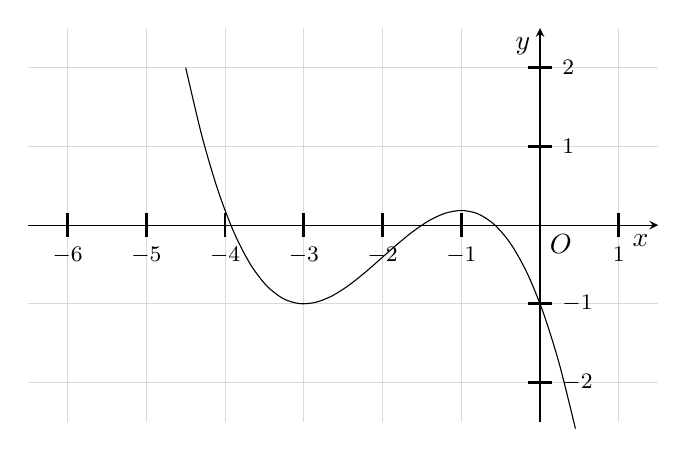
\begin{tikzpicture}[scale=1]
			\draw[step=1,gray!30,thin] (-6.5,-2.5) grid (1.5,2.5);
			\foreach \x in {-6,-5,...,-1,1}
			\draw[line width=1pt] (\x,-0.15) node[below]{ \footnotesize $\x$}--(\x,0.15) ;
			\foreach \y in {-2,-1,1,2}
			\draw[line width=1pt] (-0.15,\y)--(0.15,\y) node[right]{ \footnotesize $\y$} ;
			\draw[-stealth] (-6.5,0)--(1.5,0)node[below left]{$x$};
			\draw[-stealth] (0,-2.5)--(0,2.5)node[below left]{$y$};
			\draw[smooth,xscale=1.5] plot[domain=-3:0.3] (\x,{-(\x)^3-4 *(\x)^2-4*(\x)-1}) (0,0) node[below right]{$O$};
		\end{tikzpicture}
	\end{center}
	Có bao nhiêu số dương trong các số $a$, $b$, $c$, $d$?
	\choice
	{\True $0$}
	{$1$}
	{$2$}
	{$3$}
	\loigiai{
		Dựa vào giao điểm của đồ thị với trục tung ta có $d<0$, dựa vào dáng của đồ thị suy ra $a<0$.\\
		Ta có $y'=3ax^2+2bx+c$, dựa vào đồ thị ta có phương trình $y'=0$ có hai nghiệm phân biệt âm suy ra
		$\heva{&\dfrac{c}{3a}>0\Rightarrow c<0\\&-\dfrac{2b}{3a}<0\Rightarrow b<0.}$}
\end{ex}
\begin{ex}%Câu 49.%[2D1B5-1]
	[THPT Phan Đình Phùng - Quảng Bình - 2021] Cho hàm số $f(x)=\dfrac{ax-4}{bx+c}\left(a,b,c\in\mathbb{R}\right)$ có bảng biến thiên như sau: 
	\begin{center}
		\begin{tikzpicture}
			\tkzTabInit[nocadre=false,lgt=1.2,espcl=3.5]
			{$ x $ /0.7, $ y' $ /0.7, $ y $ /2}
			{$ -\infty $, $1 $,  $ +\infty $}
			\tkzTabLine{,+, d,+, }
			\tkzTabVar{-/$+1$,+D-/$+\infty$/$-\infty$,+/ $1$}
		\end{tikzpicture}
	\end{center}
	Trong các số $a$, $b$, $c$ có bao nhiêu số dương?
	\choice
	{$3$}
	{$0$}
	{\True $2$}
	{$1$}
	\loigiai{
		Ta có: $f(0)=-\dfrac{4}{c}>0\Rightarrow c<0$.\\
		Tiệm cận đứng của đồ thị hàm số: $x=-\dfrac{c}{b}>0\Rightarrow b>0$.\\
		Tiệm cận ngang của đồ thị hàm số: $y=\dfrac{a}{b}>0\Rightarrow a>0$.\\
		Vậy trong các số $a$, $b$, $c$ có $2$ số dương.}
\end{ex}
\begin{ex}%Câu 50.%[2D1B5-1]
	[THPT Đào Duy Từ - Hà Nội - 2021] Cho đồ thị của hàm số $f(x)=ax^4+bx^2+c$ như hình vẽ bên. Khẳng định nào sau đây là đúng?
	\begin{center}
		\begin{tikzpicture}[scale=1]
			\draw[-stealth] (-2.5,0)--(2.5,0)node[below left]{$x$};
			\draw[-stealth] (0,-1)--(0,4)node[below left]{$y$};
			\draw[smooth] plot[domain=-1.7:1.7] (\x,{(\x)^4-2*(\x)^2+1}) (0,0) node[below right]{$O$};
		\end{tikzpicture}
	\end{center}
	\choice
	{\True $a>0$; $b<0$; $c>0$; $b^2-4ac=0$}
	{$a>0$; $b>0$; $c>0$; $b^2-4ac=0$}
	{$a>0$; $b<0$; $c>0$; $b^2-4ac>0$}
	{$a>0$; $b<0$; $c>0$; $b^2-4ac<0$}
	\loigiai{
		Quan sát dáng điệu đồ thị ta thấy $a>0$, đồ thị có 3 cực trị nên $ab<0\Rightarrow b<0$.\\
		Đồ thị cắt trục tung tại điểm có tung độ dương nên $c>0$.\\
		Đồ thị tiếp xúc với trục hoành nên tại $x_1>0$ ta có\\
		$$\heva{&ax_1^4+bx_1^2+c=0\\&4ax_1^3+2bx_1=0}\Rightarrow\heva{&ax_1^4+bx_1^2+c=0\\&x_1^2=\dfrac{-b}{2a}}$$
		$\Rightarrow a\cdot\left(\dfrac{-b}{2a}\right)^2+b\cdot\dfrac{-b}{2a}+c=0\Rightarrow\dfrac{4ac-b^2}{4a}=0\Rightarrow b^2-4ac=0$.}
\end{ex}
\begin{ex}%Câu 51.%[2D1B5-1]
	[Sở Quảng Bình - 2021] Cho hàm số $y=\dfrac{ax+b}{cx+d}$ có đồ thị như hình vẽ bên dưới, trong đó $d<0$. Trong các số $a$, $b$, $c$ có bao nhiêu số dương?
	\begin{center}
		\begin{tikzpicture}[scale=1]
			\draw[-stealth] (-3.5,0)--(6,0)node[below left]{$x$};
			\draw[-stealth] (0,-4)--(0,5.5)node[below left]{$y$};
			\draw[smooth] plot[domain=-3:0.55] (\x,{((\x)+1)/((\x)-1)}) (0,0) node[below right]{$O$};
			\draw[smooth] plot[domain=1.8:5.5] (\x,{((\x)+2)/((\x)-1)});
			\draw (1,-3.8)--(1,4.8) (-3,1)--(5.5,1);
		\end{tikzpicture}
	\end{center}
	\choice
	{$0$}
	{$1$}
	{$2$}
	{\True $3$}
	\loigiai{
		\begin{center}
			\begin{tikzpicture}[scale=1]
				\draw[-stealth] (-3.5,0)--(6,0)node[below left]{$x$};
				\draw[-stealth] (0,-4)--(0,5.5)node[below left]{$y$};
				\draw[smooth] plot[domain=-3:0.55] (\x,{((\x)+1)/((\x)-1)}) (0,0) node[below right]{$O$};
				\draw[smooth] plot[domain=1.8:5.5] (\x,{((\x)+2)/((\x)-1)});
				\draw (1,-3.8)--(1,4.8) (-3,1)--(5.5,1);
				\draw (1.5, -.5) node {$-\dfrac{d}{c}$}
				(-.5,1) node[above] {$\dfrac{a}{c}$}
				(-1,-0.5) node {-$\dfrac{b}{a}$}
				;
			\end{tikzpicture}
		\end{center}
		Đồ thị có tiệm cận đứng $x=-\dfrac{d}{c}$ mà $-\dfrac{d}{c}>0\Rightarrow c>0$.\\
		Đồ thị có tiệm cận ngang $y=\dfrac{a}{c}$ mà $\dfrac{a}{c}>0\Rightarrow a>0$.\\
		Đồ thị cắt trục $Ox$ mà tại điểm có hoành độ $-\dfrac{b}{a}$ mà $-\dfrac{b}{a}<0\Rightarrow b>0$.\\
		Vậy trong các số $a$, $b$, $c$ có $3$ số dương.}
\end{ex}
\begin{ex}%Câu 52.%[2D1B5-1]
	[Sở Cần Thơ - 2021] Cho hàm số $y=\dfrac{bx-c}{x-a}$ ($a \ne 0$ và $a$, $b$, $c \in \mathbb{R}$) có đồ thị như sau: 
	\begin{center}
		\begin{tikzpicture}[scale=1]
			\foreach \x in {-3,-2,-1,1,2,...,5}
			\draw[line width=1pt] (\x,-0.15) node[below right]{ \footnotesize $\x$}--(\x,0.15) ;
			\foreach \y in {-2,-1,1,2,...,5}
			\draw[line width=1pt] (-0.15,\y)--(0.15,\y) node[below right]{ \footnotesize $\y$} ;
			\draw[-stealth] (-3.5,0)--(6,0)node[below left]{$x$};
			\draw[-stealth] (0,-4)--(0,5.5)node[below left]{$y$};
			\draw[smooth] plot[domain=-3:0.55] (\x,{((\x)+1)/((\x)-1)}) (0,0) node[below right]{$O$};
			\draw[smooth] plot[domain=1.8:5.5] (\x,{((\x)+2)/((\x)-1)});
			\draw (1,-3.8)--(1,4.8) (-3,1)--(5.5,1);
		\end{tikzpicture}
	\end{center}
	Khẳng định nào sau đây đúng?
	\choice
	{$a<0$; $b>0$; $c<0$}
	{$a<0$; $b<0$; $c>0$}
	{$a>0$; $b<0$; $c<0$}
	{\True $a>0$; $b>0$; $c<0$}
	\loigiai{
		Đồ thị hàm số $y=\dfrac{bx-c}{x-a}$ có tiệm cận đứng $x=a$, tiệm cận ngang $y=b$.\\
		Đồ thị cắt trục tung tại điểm $\left(0; \dfrac{c}{a}\right).$
		Nhìn hình vẽ ta thấy: $\heva{&a>0\\ &b > 0\\ &\dfrac{c}{a} <0} \Leftrightarrow \heva{&a>0\\ &b>0\\ &c<0.}$}
\end{ex}
\begin{ex}%Câu 53.%[2D1B5-1]
	[Sở Cần Thơ - 2021] Cho hàm số $y=ax^3+bx^2+cx+d\left(a,b,c,d\in\mathbb{R}\right)$ có đồ thị như sau: 
	\begin{center}
		\begin{tikzpicture}[scale=0.8]
			\draw[-stealth] (-3.5,0)--(2,0)node[below left]{$x$};
			\draw[-stealth] (0,-1)--(0,4.5)node[below left]{$y$};
			\draw[smooth,yscale=0.8,xscale=1.2] plot[domain=-2.8:0.6] (\x,{-(\x)^3-4*(\x)^2-4*(\x)+3}) (0,0) node[below left]{$O$};
		\end{tikzpicture}
	\end{center}
	Có bao nhiêu số dương trong các số $a$, $b$, $c$, $d$?
	\choice
	{$4$}
	{$2$}
	{$1$}
	{$3$}
	\loigiai{
		Đồ thị hàm số cắt trục tung tại điểm có tung độ dương $\Rightarrow d>0$.\\
		$\lim\limits_{x\to+\infty} y<0\Rightarrow a<0$.\\
		Ta có: $y'=3ax^2+2bx+c$.\\
		Đồ thị hàm số có 2 điểm cực trị nằm về bên trái trục tung nên phương trình $y'=0$ có 2 nghiệm phân biệt $x_1<x_2<0$.\\
		Khi đó theo Vi-ét ta có: $\heva{&x_1+x_2=-\dfrac{2b}{3a}<0\\&x_1\cdot x_2=\dfrac{c}{3a}>0}$. Từ đó suy ra $b<0$ và $c<0$.\\
		Vậy trong các số $a$, $b$, $c$, $d$ chỉ có $d>0$.}
\end{ex}
\begin{ex}%Câu 54.%[2D1B5-1]
	[Chuyên Biên Hòa - 2021] Cho hàm số $y=ax^4+bx^2+c$ có đồ thị như hình vẽ sau: 
	\begin{center}
		\begin{tikzpicture}[scale=1]
			\draw[-stealth] (-2.5,0)--(2.5,0)node[below left]{$x$};
			\draw[-stealth] (0,-1.5)--(0,3)node[below left]{$y$};
			\draw[smooth] plot[domain=-1.7:1.7] (\x,{-(\x)^4+2*(\x)^2+1}) (0,0) node[below right]{$O$};
		\end{tikzpicture}
	\end{center}
	Trong các khẳng định sau, khẳng định nào đúng?
	\choice
	{$a<0$; $b<0$; $c>0$}
	{$a>0$; $b<0$; $c>0$}
	{\True $a<0$; $b>0$; $c>0$}
	{$a>0$; $b<0$; $c<0$}
	\loigiai{
		Tập xác định: $\mathscr{D}=\mathbb{R}$. Ta có: $y'=4ax^3+2bx=2x\left(2ax^2+b\right)$.\\
		Nhìn hình dáng đồ thị ta có $a<0$.\\
		Đồ thị hàm số cắt trục tung tại điểm $M(0;c)$ nằm phía trên trục hoành nên $c>0$.\\
		Đồ thị hàm số có 3 điểm cực trị nên phương trình $y'=0$ có 3 nghiệm phân biệt. Do đó $-\dfrac{b}{2a}>0\Rightarrow b>0$.}
\end{ex}
\begin{ex}%Câu 55.%[2D1B5-1]
	[Liên Trường Nghệ An – 2021] Cho hàm số $f(x)=ax^4+bx^2+c (a,b,c\in \mathbb{R})$ có đồ thị cho bởi hình vẽ bên. Chọn khẳng định đúng: 
	\begin{center}
		\begin{tikzpicture}[scale=1]
			\draw[-stealth] (-2.5,0)--(2.5,0)node[below left]{$x$};
			\draw[-stealth] (0,-2.5)--(0,2)node[below left]{$y$};
			\draw[smooth] plot[domain=-1.7:1.7] (\x,{(\x)^4-2*(\x)^2-1}) (0,0) node[below right]{$O$};
		\end{tikzpicture}
	\end{center}
	\choice
	{$b>a$}
	{$ab+c>0$}
	{\True $a-c>0$}
	{$abc<0$}
	\loigiai{
		Ta có $\lim\limits_{x\to\pm\infty} f(x)=+\infty\Rightarrow a>0$; Hàm số có 3 điểm cực trị nên $ab<0\Rightarrow b<0$.\\
		Đồ thị hàm số cắt trục tung tại điểm nằm phía dưới trục hoành nên $c<0$.\\
		Vậy $a>0$; $b<0$; $c<0$ suy ra $a-c>0$.}
\end{ex}
\begin{ex}%Câu 56.%[2D1B5-1]
	[Chuyên Nguyễn Bỉnh Khiêm - Quảng Nam - 2021] Cho hàm số $y=ax^3+bx^2+cx+d$ có đồ thị như hình vẽ bên. Mệnh đề nào sau đây đúng?
	\begin{center}
		\begin{tikzpicture}[scale=0.8]
			\draw[-stealth] (-4,0)--(2,0)node[below left]{$x$};
			\draw[-stealth] (-2,-1.5)--(-2,3)node[below left]{$y$};
			\draw[smooth,yscale=1.2] plot[domain=-2.8:0.3] (\x,{-(\x)^3-4*(\x)^2-4*(\x)+0.5}) (-2,0) node[below left]{$O$};
		\end{tikzpicture}
	\end{center}	\choice
	{$a<0$,  $b>0$, $c>0$, $d>0$}
	{$a<0$, $b<0$, $c=0$, $d>0$}
	{\True $a<0$, $b>0$, $c=0$, $d>0$}
	{$a>0$, $b<0$, $c>0$, $d>0$}
	\loigiai{
		Nhánh cuối đồ thị đi xuống nên $a<0$.\\
		Điểm uốn lệch bên phải trục $Oy$ nên $ab<0\Rightarrow b>0$.\\
		Đồ thị có 2 cực trị trong đó một cực trị thuộc $Oy$ nên $c=0$.\\
		Đồ thị cắt trục tung tại điểm có tung độ dương nên $d>0$.}
\end{ex}
\begin{ex}%Câu 57.%[2D1B5-1]
	[Sở Cần Thơ - 2021]
	\immini{ Cho hàm số $f(x)=\dfrac{ax+2}{bx+c}$, $\left(a,b,c,d\in\mathbb{R}\right)$ có đồ thị như hình bên. Khẳng định nào dưới đây đúng?
		\choice
		{$b<a<0<c$}
		{$b<0<a<c$}
		{$a<b<0<c$}
		{$b<0<c<a$}}{
		\begin{tikzpicture}[>=stealth]
			\def\xmin{-2}\def\xmax{4}\def\ymin{-1}\def\ymax{5}
			\draw[->](\xmin,0)--(\xmax,0)node [shift={(-90:.2)},scale=1]{\scriptsize $x$};
			\draw[->](0,\ymin)--(0,\ymax)node [below left] {\scriptsize $y$};
			\clip(\xmin,\ymin) rectangle (\xmax,\ymax);
			\foreach \p/\g in {1/-45}\draw(\p,0)node[shift={(\g:.2)},scale=1]{\scriptsize $\p$}--+(0,.05)--+(0,-.05);
			\foreach \p/\g in {1/180, 2/135}\draw(0,\p)node[shift={(\g:.3)},scale=1]{\scriptsize $\p$}--+(.05,0)--+(-.05,0);
			\foreach \p/\g in {0/-135}\draw(0,\p)node[shift={(\g:.3)},scale=1]{\scriptsize $O$};
			\draw[thick,blue,smooth,samples=100] plot[domain=\xmin:0.99](\x,{(-4*\x+2)/(-2*\x+2)})node[left]{\scriptsize };
			\draw[thick,blue,smooth,samples=100] plot[domain=1.01:\xmax](\x,{(-4*\x+2)/(-2*\x+2)})node[left]{\scriptsize };
			\draw[dashed](\xmin,2)--(\xmax,2)(1,\ymin)--(1,\ymax);
		\end{tikzpicture}
	}
	\loigiai{
		Khi $x=0\Rightarrow y=\dfrac{2}{c}=1\Rightarrow c=2$.\\
		Tiệm cận đứng $x=-\dfrac{c}{b}=1\Rightarrow-\dfrac{2}{b}=1\Rightarrow b=-2$.\\
		Tiệm cận ngang $y=\dfrac{a}{b}=2\Rightarrow\dfrac{a}{-2}=2\Rightarrow a=-4$.\\
		Vậy $a<b<0<c$.}
\end{ex}
\begin{ex}%Câu 58.%[2D1B5-5]
	[Sở Thái Nguyên 2022] 
	\immini{Cho hàm số $y=f(x)=\dfrac{ax+b}{cx+d}$ có đồ thị hàm số $f'(x)$ như trong hình vẽ bên. Biết rằng đồ thị hàm số $f(x)$ đi qua điểm $A(0;2)$. Giá trị $f(3)$ bằng
		\choice
		{$-2$}
		{$-1$}
		{$3$}
		{\True $5$}}{
		\begin{tikzpicture}[>=stealth]
			\def\xmin{-1}\def\xmax{5}\def\ymin{-4}\def\ymax{1}
			\draw[->](\xmin,0)--(\xmax,0)node [shift={(-90:.2)},scale=1]{\scriptsize $x$};
			\draw[->](0,\ymin)--(0,\ymax)node [below left] {\scriptsize $y$};
			\clip(\xmin,\ymin) rectangle (\xmax,\ymax);
			\foreach \p/\g in {2/45}\draw(\p,0)node[shift={(\g:.2)},scale=1]{\scriptsize $\p$}--+(0,.05)--+(0,-.05);
			\foreach \p/\g/\t in {-0.5/-135/-\frac12}\draw(0,\p)node[shift={(\g:.3)},scale=1]{\scriptsize $\t$}--+(.05,0)--+(-.05,0);
			\foreach \p/\g in {0/45}\draw(0,\p)node[shift={(\g:.3)},scale=1]{\scriptsize $O$};
			\draw[thick,blue,smooth,samples=100] plot[domain=\xmin:1.9](\x,{-2/((\x-2)^2)})node[left]{\scriptsize };
			\draw[thick,blue,smooth,samples=100] plot[domain=2.1:\xmax](\x,{-2/((\x-2)^2)})node[left]{\scriptsize };
			\draw(2,\ymin)--(2,\ymax);
		\end{tikzpicture}	
	}
	\loigiai{
		Ta có $y=f(x)=\dfrac{ax+b}{cx+d}\Rightarrow f'(x)=\dfrac{ad-bc}{(cx+d)^2}$.\\
		Vì đồ thị thị hàm số $f(x)$ đi qua điểm $A(0;2)$ suy ra $f(0)=2\Rightarrow\dfrac{b}{d}=2\Leftrightarrow b=2d$.\hfill(1)\\
		Dựa vào đồ thị hàm số $f'(x)$ ta có: $\heva{&f'(0)=-\dfrac{1}{2}\\&x=-\dfrac{d}{c}=2}\Rightarrow\heva{&\dfrac{ad-bc}{d^2}=-\dfrac{1}{2}&(2)\\&d=-2c.&(3)}$ \\
		Thay $(1)$ vào $(2)$: 
		$$\dfrac{ad-2dc}{d^2}=-\dfrac{1}{2}\Rightarrow\dfrac{a-2c}{d}=-\dfrac{1}{2}\Rightarrow a=-\dfrac{1}{2}d+2c=-\dfrac{1}{2}\cdot (-2c)+2c=3c.$$
		Vậy, $f(3)=\dfrac{3a+b}{3c+d}=\dfrac{3\cdot 3c-4c}{3c-2c}=\dfrac{5c}{c}=5$.		 
	}
\end{ex}
\begin{dang}
	{Đồ thị hàm số chứa dấu giá trị tuyệt đối, biến đổi đồ thị}
\end{dang}
\begin{dang}{Từ đồ thị $(C)\colon y=f(x)$ suy ra đồ thị $(C')\colon y=\left|f(x)\right|$.}
	Ta có $y=\left|f(x)\right|=\heva{&f(x)\text{ khi }f(x)\geq 0\\&-f(x)\text{ khi }f(x)<0.}$ \\
	Cách vẽ $(C')$ từ $(C)$:
	\begin{itemize}
		\item Giữ nguyên phần đồ thị phía trên $Ox$ của đồ thị $(C)$: $y=f(x)$.
		\item Bỏ phần đồ thị phía dưới $Ox$ của $(C)$, lấy đối xứng phần đồ thị bị bỏ qua $Ox$. 
	\end{itemize}
\end{dang}
\begin{vd}%[2D1B5-2]
	Từ đồ thị $(C)\colon y=f(x)=x^3-3x$ suy ra đồ thị $y=\left|x^3-3x\right|$.
	\loigiai{
		Biến đổi $(C)$:
		\begin{itemize}
			\item Bỏ phần đồ thị của $(C)$ dưới $Ox$, giữ nguyên $(C)$ phía trên $Ox$.
			\item Lấy đối xứng phần đồ thị bị bỏ qua $Ox$.
		\end{itemize}
		\begin{center}
			\begin{tabular}{cc}
				\begin{tikzpicture}[>=stealth]
					\def\xmin{-2.5}\def\xmax{2.5}\def\ymin{-3}\def\ymax{3}
					\draw[->](\xmin,0)--(\xmax,0)node [shift={(-90:.2)},scale=1]{\scriptsize $x$};
					\draw[->](0,\ymin)--(0,\ymax)node [below left] {\scriptsize $y$};
					\clip(\xmin,\ymin) rectangle (\xmax,\ymax);
					\foreach \p/\g in {1/90,-1/-90}\draw(\p,0)node[shift={(\g:.2)},scale=1]{\scriptsize $\p$}--+(0,.05)--+(0,-.05);
					\foreach \p/\g in {-2/180,2/45}\draw(0,\p)node[shift={(\g:.3)},scale=1]{\scriptsize $\p$}--+(.05,0)--+(-.05,0);
					\foreach \p/\g in {0/-135}\draw(0,\p)node[shift={(\g:.3)},scale=1]{\scriptsize $O$};
					\draw[thick,blue,smooth,samples=100] plot[domain=\xmin:\xmax](\x,{(\x)^3-3*(\x)})node[left]{\scriptsize};
					\draw[dashed](-1,0)--(-1,2)--(0,2)(1,0)--(1,-2)--(0,-2);
				\end{tikzpicture}
				&
				\begin{tikzpicture}[>=stealth]
					\def\xmin{-2.5}\def\xmax{2.5}\def\ymin{-3}\def\ymax{3}
					\draw[->](\xmin,0)--(\xmax,0)node [shift={(-90:.2)},scale=1]{\scriptsize $x$};
					\draw[->](0,\ymin)--(0,\ymax)node [below left] {\scriptsize $y$};
					\clip(\xmin,\ymin) rectangle (\xmax,\ymax);
					\foreach \p/\g in {1/-90,-1/-90}\draw(\p,0)node[shift={(\g:.2)},scale=1]{\scriptsize $\p$}--+(0,.05)--+(0,-.05);
					\foreach \p/\g in {-2/-180,2/45}\draw(0,\p)node[shift={(\g:.3)},scale=1]{\scriptsize $\p$}--+(.05,0)--+(-.05,0);
					\foreach \p/\g in {0/-135}\draw(0,\p)node[shift={(\g:.3)},scale=1]{\scriptsize $O$};
					\draw[thick,blue,smooth,samples=100] plot[domain=\xmin:\xmax](\x,{abs((\x)^3-3*(\x))})node[left]{\scriptsize};
					\draw[dashed](-1,0)--(-1,2)--(1,2)--(1,0);
				\end{tikzpicture}
				\cr
				$(C):y=x^3-3x$&$(C'):y=|x^3-3x|$
			\end{tabular}
		\end{center}
	}
\end{vd}
\begin{dang}{Từ đồ thị $(C)\colon y=f(x)$ suy ra đồ thị $(C')\colon y=f(|x|)$}
\end{dang}
\begin{ex}%[2D1B5-2]
	Từ đồ thị $(C)\colon y=f(x)=x^3-3x$ suy ra đồ thị $(C')\colon y=|x|^3-3|x|$.
	\loigiai{
		Biến đổi $(C)$:
		\begin{itemize}
			\item Giữ nguyên phần đồ thị bên phải $Oy$ của đồ thị $(C)\colon y=f(x)$.
			\item Bỏ phần đồ thị bên trái $Oy$ của $(C)$, lấy đối xứng phần đồ thị được giữ qua $Oy$. 
		\end{itemize}
		\begin{center}
			\begin{tabular}{cc}
				\begin{tikzpicture}[>=stealth]
					\def\xmin{-2.5}\def\xmax{2.5}\def\ymin{-3}\def\ymax{3}
					\draw[->](\xmin,0)--(\xmax,0)node [shift={(-90:.2)},scale=1]{\scriptsize $x$};
					\draw[->](0,\ymin)--(0,\ymax)node [below left] {\scriptsize $y$};
					\clip(\xmin,\ymin) rectangle (\xmax,\ymax);
					\foreach \p/\g in {1/90,-1/-90}\draw(\p,0)node[shift={(\g:.2)},scale=1]{\scriptsize $\p$}--+(0,.05)--+(0,-.05);
					\foreach \p/\g in {-2/180,2/0}\draw(0,\p)node[shift={(\g:.3)},scale=1]{\scriptsize $\p$}--+(.05,0)--+(-.05,0);
					\foreach \p/\g in {0/-135}\draw(0,\p)node[shift={(\g:.3)},scale=1]{\scriptsize $O$};
					\draw[thick,blue,smooth,samples=100] plot[domain=\xmin:\xmax](\x,{(\x)^3-3*(\x)})node[left]{\scriptsize};
					\draw[dashed](-1,0)--(-1,2)--(0,2)(1,0)--(1,-2)--(0,-2);
				\end{tikzpicture}
				&
				\begin{tikzpicture}[>=stealth]
					\def\xmin{-2.5}\def\xmax{2.5}\def\ymin{-3}\def\ymax{3}
					\draw[->](\xmin,0)--(\xmax,0)node [shift={(-90:.2)},scale=1]{\scriptsize $x$};
					\draw[->](0,\ymin)--(0,\ymax)node [below left] {\scriptsize $y$};
					\clip(\xmin,\ymin) rectangle (\xmax,\ymax);
					\foreach \p/\g in {1/90,-1/90}\draw(\p,0)node[shift={(\g:.2)},scale=1]{\scriptsize $\p$}--+(0,.05)--+(0,-.05);
					\foreach \p/\g in {-2/135,2/0}\draw(0,\p)node[shift={(\g:.3)},scale=1]{\scriptsize $\p$}--+(.05,0)--+(-.05,0);
					\foreach \p/\g in {0/45}\draw(0,\p)node[shift={(\g:.3)},scale=1]{\scriptsize $O$};
					\draw[thick,blue,smooth,samples=100] plot[domain=\xmin:\xmax](\x,{abs(\x)^3-3*abs(\x)})node[left]{\scriptsize};
					\draw[dashed](-1,0)--(-1,-2)--(1,-2)--(1,0);
				\end{tikzpicture}
				\cr
				$(C):y=x^3-3x$&$(C'):y=|x|^3-3|x|$
			\end{tabular}
		\end{center}
	}
\end{ex}
\begin{ex}%[2D1B5-2]
	Từ đồ thị $(C)\colon y=f(x)=x^3-3x$ suy ra đồ thị $y=\left||x|^3-3|x|\right|$.
	\loigiai{
		Biến đổi $(C)$ để được đồ thị $(C')\colon y=|x|^3-3|x|$. Biến đổi $(C')\colon y=|x|^3-3|x|$ ta được đồ thị $(C'')\colon y=\left||x|^3-3|x|\right|$.
		\begin{center}
			\begin{tikzpicture}[>=stealth]
				\def\xmin{-2.5}\def\xmax{2.5}\def\ymin{-3}\def\ymax{3}
				\draw[->](\xmin,0)--(\xmax,0)node [shift={(-90:.2)},scale=1]{\scriptsize $x$};
				\draw[->](0,\ymin)--(0,\ymax)node [below left] {\scriptsize $y$};
				\clip(\xmin,\ymin) rectangle (\xmax,\ymax);
				\foreach \p/\g in {1/-90,-1/-90}\draw(\p,0)node[shift={(\g:.2)},scale=1]{\scriptsize $\p$}--+(0,.05)--+(0,-.05);
				\foreach \p/\g in {-2/180,2/45}\draw(0,\p)node[shift={(\g:.3)},scale=1]{\scriptsize $\p$}--+(.05,0)--+(-.05,0);
				\foreach \p/\g in {0/-135}\draw(0,\p)node[shift={(\g:.3)},scale=1]{\scriptsize $O$};
				\draw[thick,blue,smooth,samples=100] plot[domain=\xmin:\xmax](\x,{abs(abs(\x)^3-3*abs(\x))})node[left]{\scriptsize};
				\draw[dashed](-1,0)--(-1,2)--(1,2)--(1,0);
			\end{tikzpicture}
		\end{center}
	}
\end{ex}
\begin{dang}{Từ đồ thị $(C)\colon y=u(x)\cdot v(x)$ suy ra đồ thị $(C')\colon y=\left|u(x)\right|\cdot v(x)$}
\end{dang}

\begin{ex}%[2D1B5-2]
	Từ đồ thị $(C)\colon y=f(x)=2x^3-3x^2+1$ suy ra đồ thị $(C')\colon y=|x-1|(2x^2-x-1)$.
	\loigiai{
		\immini{$$y=|x-1|\left(2x^2-x-1\right)=\heva{&f(x)\text{ khi }x\geq 1\\&-f(x)\text{ khi }x<1.}$$
			Đồ thị $(C')$:
			\begin{itemize}
				\item Giữ nguyên $(C)$ với $x\geq 1$.
				\item Bỏ $(C)$ với $x<1$. Lấy đối xứng phần đồ thị bị bỏ qua $Ox$. 
			\end{itemize}
			Nhận xét: Trong quá trình thực hiện phép suy đồ thị nên lấy đối xứng các điểm đặc biệt của $(C)$: giao điểm với $Ox$, $Oy$, CĐ, CT…	 
		}{
			\begin{tikzpicture}[>=stealth]
				\def\xmin{-2.5}\def\xmax{2.5}\def\ymin{-3}\def\ymax{3}
				\draw[->](\xmin,0)--(\xmax,0)node [shift={(-90:.2)},scale=1]{\scriptsize $x$};
				\draw[->](0,\ymin)--(0,\ymax)node [below left] {\scriptsize $y$};
				\clip(\xmin,\ymin) rectangle (\xmax,\ymax);
				\foreach \p/\g in {1/-90}\draw(\p,0)node[shift={(\g:.2)},scale=1]{\scriptsize $\p$}--+(0,.05)--+(0,-.05);
				\foreach \p/\g in {-1/-135}\draw(0,\p)node[shift={(\g:.3)},scale=1]{\scriptsize $\p$}--+(.05,0)--+(-.05,0);
				\foreach \p/\g in {0/-135}\draw(0,\p)node[shift={(\g:.3)},scale=1]{\scriptsize $O$};
				\draw[dashed,blue,smooth,samples=100] plot[domain=\xmin:\xmax](\x,{2*(\x)^3-3*(\x)^2+1})node[left]{\scriptsize};
				\draw[thick,blue,smooth,samples=100] plot[domain=\xmin:\xmax](\x,{abs(\x-1)*(2*(\x)^2-\x-1)})node[left]{\scriptsize};
			\end{tikzpicture}
		}
	}
\end{ex}

\begin{ex}%[2D1B5-2]
	Từ đồ thị $(C)\colon y=f(x)=\dfrac{x}{x-1}$ suy ra đồ thị $(C')\colon y=\dfrac{x}{|x-1|}$.
	\loigiai{
		\immini{
			$$y=\dfrac{x}{|x-1|}=\heva{&\dfrac{x}{x-1}\text{ khi }x\in(1;+\infty)\\&-\dfrac{x}{x-1}\text{ khi }x\in(-\infty;1).}$$
			Đồ thị $(C')$:
			\begin{itemize}
				\item Bỏ phần đồ thị của $(C)$ với $x<1$, giữ nguyên $(C)$ với $x>1$.
				\item Lấy đối xứng phần đồ thị bị bỏ qua $Ox$.
			\end{itemize}
			Nhận xét: Đối với hàm phân thức thì nên lấy đối xứng các đường tiệm cận để thực hiện phép suy đồ thị một cách tương đối chính xác.
		}{
			\begin{tikzpicture}[>=stealth]
				\def\xmin{-1}\def\xmax{3}\def\ymin{-3}\def\ymax{3}
				\draw[->](\xmin,0)--(\xmax,0)node [shift={(-90:.2)},scale=1]{\scriptsize $x$};
				\draw[->](0,\ymin)--(0,\ymax)node [below left] {\scriptsize $y$};
				\clip(\xmin,\ymin) rectangle (\xmax,\ymax);
				\foreach \p/\g in {1/-45}\draw(\p,0)node[shift={(\g:.2)},scale=1]{\scriptsize $\p$}--+(0,.05)--+(0,-.05);
				\foreach \p/\g in {1/-135,-1/-135}\draw(0,\p)node[shift={(\g:.3)},scale=1]{\scriptsize $\p$}--+(.05,0)--+(-.05,0);
				\foreach \p/\g in {0/-45}\draw(0,\p)node[shift={(\g:.3)},scale=1]{\scriptsize $O$};
				\draw[thick,blue,smooth,samples=100] plot[domain=\xmin:0.99](\x,{\x/abs(\x-1)})node[left]{\scriptsize};
				\draw[thick,blue,smooth,samples=100] plot[domain=1.01:\xmax](\x,{\x/abs(\x-1)})node[left]{\scriptsize};
				\draw(1,\ymin)--(1,\ymax)(\xmin,1)--(\xmax,1)(\xmin,-1)--(\xmax,-1);
			\end{tikzpicture}
		}
	}
\end{ex}

\begin{ex}%Câu 1.%[2D1B5-2]
	Cho hàm số $y=x^3-3x^2+2$ có đồ thị như hình 1. Đồ thị hình 2 là của hàm số nào dưới đây?
	\begin{center}
		\begin{tabular}{cc}
			\begin{tikzpicture}[>=stealth]
				\def\xmin{-1}\def\xmax{3}\def\ymin{-2.5}\def\ymax{2.5}
				\draw[->](\xmin,0)--(\xmax,0)node [shift={(-90:.2)},scale=1]{\scriptsize $x$};
				\draw[->](0,\ymin)--(0,\ymax)node [below left] {\scriptsize $y$};
				\clip(\xmin,\ymin) rectangle (\xmax,\ymax);
				\foreach \p/\g in {1/45, 2/90}\draw(\p,0)node[shift={(\g:.2)},scale=1]{\scriptsize $\p$}--+(0,.05)--+(0,-.05);
				\foreach \p/\g in {-2/180, 2/45}\draw(0,\p)node[shift={(\g:.3)},scale=1]{\scriptsize $\p$}--+(.05,0)--+(-.05,0);
				\foreach \p/\g in {0/-45}\draw(0,\p)node[shift={(\g:.3)},scale=1]{\scriptsize $O$};
				\draw[thick,blue,smooth,samples=100] plot[domain=\xmin:\xmax](\x,{(\x)^3-3*(\x)^2+2})node[left]{\scriptsize};
				\draw[dashed](0,-2)--(2,-2)--(2,0);
			\end{tikzpicture}
			&
			\begin{tikzpicture}[>=stealth]
				\def\xmin{-1}\def\xmax{3}\def\ymin{-2.5}\def\ymax{2.5}
				\draw[->](\xmin,0)--(\xmax,0)node [shift={(-90:.2)},scale=1]{\scriptsize $x$};
				\draw[->](0,\ymin)--(0,\ymax)node [below left] {\scriptsize $y$};
				\clip(\xmin,\ymin) rectangle (\xmax,\ymax);
				\foreach \p/\g in {1/90, 2/90}\draw(\p,0)node[shift={(\g:.2)},scale=1]{\scriptsize $\p$}--+(0,.05)--+(0,-.05);
				\foreach \p/\g in {-2/-45, 2/45}\draw(0,\p)node[shift={(\g:.3)},scale=1]{\scriptsize $\p$}--+(.05,0)--+(-.05,0);
				\foreach \p/\g in {0/-45}\draw(0,\p)node[shift={(\g:.3)},scale=1]{\scriptsize $O$};
				\draw[thick,blue,smooth,samples=100] plot[domain=\xmin:\xmax](\x,{abs(\x-1)*((\x)^2-2*(\x)-2})node[left]{\scriptsize};
				\draw[dashed](0,-2)--(2,-2)--(2,0);
			\end{tikzpicture}\cr
			Hình 1&Hình 2
		\end{tabular}
	\end{center}
	\choice
	{$y=\left|x^3-3x^2+2\right|$}
	{$y=|x|^3-3x^2+2$}
	{\True $y=|x-1|\left(x^2-2x-2\right)$}
	{$y=(x-1)\left|x^2-2x-2\right|$}
	\loigiai{
		Ta có $y=x^3-3x^2+2=(x-1)\left(x^2-2x-2\right)$.\\
		Từ đồ thị ban đầu (hình 1) sang đồ thị thứ 2 (hình 2) ta thấy.\\
		Toàn bộ đồ thị ứng với $x\geq 1$ được giữ nguyên.\\
		Phần đồ thị ứng với $x<1$ lấy đối xứng qua trục hoành.}
\end{ex}
\begin{ex}%Câu 2.%[2D1B5-2]
	[Đề Tham Khảo 2017]
	Hàm số $y=f(x)=(x-2)(x^2-1)$ có đồ thị như hình dưới đây:
	\begin{center}
		\begin{tikzpicture}[scale=.8, font=\footnotesize, line join=round, line cap=round, >=stealth]
			%\draw[gray!30] (-2,-2) grid (3,3);
			\def\xt{-2} \def\xp{3} \def\yt{3} \def\yd{-2} % x_trái, x_phải, y_trên, y_dưới (giới hạn)
			\draw[->] (\xt,0)--(\xp,0) node [below]{$x$};
			\draw[->] (0,\yd)--(0,\yt) node [below left]{$y$};
			\node at (0,0) [below left]{$O$}; \node at (1,0) [below left]{$1$}; \node at (-1,0) [below left]{$-1$};\node at (0,2) [above right]{$2$};\node at (2,0) [below right]{$2$};
			\clip (\xt-0.1,\yd+0.1) rectangle (\xp-0.1,\yt-0.1);
			\draw[smooth,samples=350,domain=\xt+0.01:\xp-0.01,variable=\x] plot(\x,{(\x-2)*((\x)^2-1)});
			\foreach \i in {0,1,2,-1}
			\draw[fill=black] (\i,0) circle(1pt);
			\foreach \j in {2}
			\draw[fill=black] (0,\j) circle(1pt);
		\end{tikzpicture}
	\end{center}
	Hình nào dưới đây là đồ thị của hàm số $y=|x-2|(x^2-1)$?\\
	\begin{minipage}[b]{0.24\textwidth}
		\begin{center}
			\begin{tikzpicture}[scale=.8, font=\footnotesize, line join=round, line cap=round, >=stealth]
				\def \xmin{-2.5}
				\def \xmax{3}
				\def \ymin{-3}
				\def \ymax{3}
				\def \hamsot{(\x)^3-2*(\x)^2-(\x)+2}
				\def \hamsop{-(\x)^3+2*(\x)^2+(\x)-2}
				\draw[->] (\xmin,0)--(-1,0) node[below left]{$-1$}--(0,0) node [below left] {$O$}--(1,0) node[below left]{$1$}--(2,0) node[below]{$2$}--(\xmax,0) node[below left] {$x$};
				\draw[->] (0,\ymin)--(0,-2) node[right]{$-2$}--(0,\ymax) node[below left] {$y$};
				\tkzDefPoints{-1/0/A,1/0/B,2/0/C,0/-2/D}
				\tkzDrawPoints[fill=black](A,B,C,D)
				\begin{scope}
					\clip (\xmin+0.1,\ymin+0.1) rectangle (\xmax-0.1,\ymax-0.1);
					\draw[samples=350,domain=\xmin+0.1:2,smooth,variable=\x] plot (\x,{\hamsop});
					\draw[samples=350,domain=0+\xmax-0.1:2,smooth,variable=\x] plot (\x,{\hamsot});
				\end{scope}
			\end{tikzpicture}
			Hình 1
		\end{center}
	\end{minipage}
	\begin{minipage}[b]{0.24\textwidth}
		\begin{center}
			\begin{tikzpicture}[scale=.8, font=\footnotesize, line join=round, line cap=round, >=stealth]
				\def \xmin{-2.5}
				\def \xmax{3}
				\def \ymin{-3}
				\def \ymax{3}
				\def \hamsot{(\x)^3-2*(\x)^2-(\x)+2}
				\def \hamsop{-(\x)^3+2*(\x)^2+(\x)-2}
				\draw[->] (\xmin,0)--(-1,0) node[below left]{$-1$}--(0,0) node [below left] {$O$}--(1,0) node[below left]{$1$}--(2,0) node[below]{$2$}--(\xmax,0) node[below left] {$x$};
				\draw[->] (0,\ymin)--(0,-2) node[right]{$-2$}--(0,\ymax) node[below left] {$y$};
				\tkzDefPoints{-1/0/A,1/0/B,2/0/C,0/-2/D}
				\tkzDrawPoints[fill=black](A,B,C,D)
				\begin{scope}
					\clip (\xmin+0.1,\ymin+0.1) rectangle (\xmax-0.1,\ymax-0.1);
					\draw[samples=350,domain=\xmin+0.1:1,smooth,variable=\x] plot (\x,{\hamsop});
					\draw[samples=350,domain=0+\xmax-0.1:1,smooth,variable=\x] plot (\x,{\hamsot});
				\end{scope}
			\end{tikzpicture}
			Hình 2
		\end{center}
	\end{minipage}
	\begin{minipage}[b]{0.24\textwidth}
		\begin{center}
			\begin{tikzpicture}[scale=.8, font=\footnotesize, line join=round, line cap=round, >=stealth]
				\def \xmin{-3}
				\def \xmax{3}
				\def \ymin{-1.5}
				\def \ymax{3}
				\def \hamsot{(\x)^3-2*(\x)^2-(\x)+2}
				\def \hamsop{-(\x)^3-2*(\x)^2+(\x)+2}
				\draw[->] (\xmin,0)--(-2,0) node[below left]{$-2$}--(-1,0) node[below left]{$-1$}--(0,0) node [below left] {$O$}--(1,0) node[below left]{$1$}--(2,0) node[below]{$2$}--(\xmax,0) node[below left] {$x$};
				\draw[->] (0,\ymin)--(0,1) node[right]{$1$}--(0,2) node[right]{$2$}--(0,\ymax) node[below left] {$y$};
				\tkzDefPoints{-2/0/A,-1/0/B,1/0/E,2/0/C,0/1/D,0/2/F}
				\tkzDrawPoints[fill=black](A,B,C,D,E,F)
				\begin{scope}
					\clip (\xmin+0.1,\ymin+0.1) rectangle (\xmax-0.1,\ymax-0.1);
					\draw[samples=350,domain=\xmin+0.1:0,smooth,variable=\x] plot (\x,{\hamsop});
					\draw[samples=350,domain=0+\xmax-0.1:0,smooth,variable=\x] plot (\x,{\hamsot});
				\end{scope}
			\end{tikzpicture}
			Hình 3
		\end{center}
	\end{minipage}
	\begin{minipage}[b]{0.24\textwidth}
		\begin{center}
			\begin{tikzpicture}[scale=.8, font=\footnotesize, line join=round, line cap=round, >=stealth]
				\def \xmin{-2}
				\def \xmax{3}
				\def \ymin{-1}
				\def \ymax{3}
				\def \hamsot{(\x)^3-2*(\x)^2-(\x)+2}
				\def \hamsop{-(\x)^3+2*(\x)^2+(\x)-2}
				\draw[->] (\xmin,0)--(-1,0) node[below left]{$-1$}--(0,0) node [below left] {$O$}--(1,0) node[below left]{$1$}--(2,0) node[below]{$2$}--(\xmax,0) node[below left] {$x$};
				\draw[->] (0,\ymin)--(0,1) node[right]{$1$}--(0,2) node[right]{$2$}--(0,\ymax) node[below left] {$y$};
				\tkzDefPoints{-1/0/B,1/0/E,2/0/C,0/1/D,0/2/F}
				\tkzDrawPoints[fill=black](B,C,D,E,F)
				\begin{scope}
					\clip (\xmin+0.1,\ymin+0.1) rectangle (\xmax-0.1,\ymax-0.1);
					\draw[samples=350,domain=1:2,smooth,variable=\x] plot (\x,{\hamsop});
					\draw[samples=350,domain=0+\xmax-0.1:2,smooth,variable=\x] plot (\x,{\hamsot});
					\draw[samples=350,domain=-1:1,smooth,variable=\x] plot (\x,{\hamsot});
					\draw[samples=350,domain=0+\xmin+0.1:-1,smooth,variable=\x] plot (\x,{\hamsop});
				\end{scope}
			\end{tikzpicture}
			Hình 4
		\end{center}
	\end{minipage}
	\choice
	{\True Hình 1}
	{Hình 2}
	{Hình 3}
	{Hình 4}
	\loigiai{
		Ta có $y=|x-2|\left(x^2-1\right)=\heva{&(x-2)\left(x^2-1\right),x\geq 2\\&-(x-2)\left(x^2-1\right),x<2}$ nên đồ thị gồm 2 phần:\\
		+) Giữ nguyên phần đồ thị đã cho ứng với $x\geq 2$.\\
		+) Lấy đối xứng phần đồ thị đã cho ứng với $x<2$ qua trục $Ox$.\\
		Hình 1 nhận vì đồ thị là hàm $y=|x-2|\left(x^2-1\right)$.\\
		Hình 2 loại vì đồ thị là hàm $y=(x-2)|x-1|(x+1)$.\\
		Hình 3 loại vì đồ thị hàm số $y=(|x|-2)\left(x^2-1\right)$.\\
		Hình 4 loại vì đồ thị hàm $y=\left|(x-2)\left(x^2-1\right)\right|$.}
\end{ex}
\begin{ex}%Câu 3.%[2D1K2-2]
	[THPT Việt Đức Hà Nội 2019]
	\immini{ Cho hàm số $y=f(x)$ có đồ thị hàm số $y=f(|x|)$ như hình vẽ. 
		Chọn kết luận đúng trong các kết luận sau: 
		\choice
		{\True $f(x)=-x^3+x^2+4x-4$}
		{$f(x)=x^3-x^2-4x+4$}
		{$f(x)=-x^3-x^2+4x-4$}
		{$f(x)=x^3+x^2-4x-4$}}{\begin{tikzpicture}[scale=0.7, font=\footnotesize,line join=round, line cap=round, >=stealth]
			\draw[->,line width = 1pt] (-3,0)--(0,0) node[below left]{$O$}--(3,0) node[below]{$x$};
			\draw[->,line width = 1pt] (0,-4.5)--(0,2) node[left]{$y$};
			\draw[samples=100,domain=-2.6:2.6,smooth] plot (\x, {-1*abs((\x))^3+abs((\x))^2+4*abs((\x))-4});
			\draw[fill] (-2,0) circle (2pt) node [below left]{$-2$};
			\draw[fill] (-1,0)circle (2pt) node [below left]{$-1$};
			\draw[fill] (1,0)circle (2pt) node [above left]{$1$};
			\draw[fill] (2,0)circle (2pt) node [above right]{$2$};
			\draw[fill] (0,-4)circle (2pt) node [left]{$ -4 $};
	\end{tikzpicture}}
	\loigiai{
		Do đồ thị giao với trục $Oy$ tại điểm có tung độ bằng $-4$ và $\lim\limits_{x\to+\infty} y=-\infty$.}
\end{ex}
\begin{ex}%Câu 4.%[2D1K2-2]
	Biết phương trình $ax^3+bx^2+cx+d=0 (a\neq 0)$ có đúng hai nghiệm thực. Hỏi đồ thị hàm số $y=\left|ax^3+bx^2+cx+d\right|$ có bao nhiêu điểm cực trị?
	\choice
	{$4$}
	{$5$}
	{$2$}
	{\True $3$}
	\loigiai{
		Phương trình $ax^3+bx^2+cx+d=0\ (a\neq 0)$ có 2 nghiệm thực nên đồ thị hàm số $y=ax^3+bx^2+cx+\mathrm{d}\ (a\neq 0)$ dạng: 
		\begin{center}
			\begin{tikzpicture}[scale=0.6, line join=round, line cap=round,>=stealth]
				\draw [->] (-3,0) -- (4.5,0) node[below]{$x$};
				\draw [->] (0,-1) -- (0,5) node[right]{$y$};				
				\draw  plot[domain=-2.2:3.5, samples=100, smooth](\x,{0.4*(\x- 2)^2*(\x+2)});
				\begin{scope}[shift={(9,0)}]
					\draw [->] (-3,0) -- (4.5,0) node[below]{$x$};
					\draw [->] (0,-1) -- (0,5) node[right]{$y$};				
					\draw  plot[domain=-2.2:3.5, samples=100, smooth](-\x,{0.4*(\x- 2)^2*(\x+2)});
				\end{scope}
			\end{tikzpicture}
		\end{center}
		Ta có:\\
		Phương trình $ax^3+bx^2+cx+d=0 (a\neq 0)$ có đúng hai nghiệm thực.\\
		Nên đồ thị hàm số $y=ax^3+bx^2+cx+d$ được minh họa như hình vẽ.\\
		Gọi m là số điểm cực trị của hàm số $y=f(x)$ và k là nghiệm bội lẻ.\\
		của phương trình $f(x)=0$ \\
		$ \Rightarrow $ Số điểm cực trị của đồ thị hàm số $y=\left|f(x)\right|$ là $m+k$.\\
		Vậy đồ thị hàm số $y=\left|ax^3+bx^2+cx+d\right|$ có số điểm cực trị là $2+1$.}
\end{ex}
\begin{ex}%Câu 5.%[2D1B5-2]
	[Chu Văn An - Hà Nội - 2019] Cho hàm số $y=(x-2)\left(x^2-1\right)$ có đồ thị như hình vẽ:
	\begin{center}
		\begin{tikzpicture}[scale=0.7, font=\footnotesize,line join=round, line cap=round, >=stealth]
			\def \xmin{-2}
			\def \xmax{3}
			\def \ymin{-1}
			\def \ymax{3}
			\def \hamso{(\x-2)*((\x)^2-1)}
			\draw[->] (\xmin,0)--(\xmax,0) node[below] {$x$};
			\draw[->] (0,\ymin)--(0,\ymax) node[left] {$y$};
			\draw (0,0) node [below left] {$O$};
			\begin{scope}
				\clip (\xmin,\ymin) rectangle (\xmax,\ymax);
				\draw[smooth,samples=200,domain=-2.5:2.5] plot (\x,{\hamso});
				\foreach \x/\y/\pos/\n in {-1/0/below left/-1,1/0/below left/1,2/0/below right/2} \fill (\x,\y)node[\pos]{$\n$} circle(1.5pt);
			\end{scope}
		\end{tikzpicture}
	\end{center}
	Một trong bốn hình dưới đây là đồ thị của hàm số $y=(x-2)\left|x^2-1\right|$. Hỏi đó là hình nào?\\
	\begin{minipage}{0.24\textwidth}
		\begin{center}
			\begin{tikzpicture}[scale=0.7, font=\footnotesize,line join=round, line cap=round, >=stealth]
				\def \xmin{-2}
				\def \xmax{3}
				\def \ymin{-2.5}
				\def \ymax{3}
				\def \hamso{abs((\x)-2)*((\x)^2-1)}
				\draw[->] (\xmin,0)--(\xmax,0) node[below] {$x$};
				\draw[->] (0,\ymin)--(0,\ymax) node[left] {$y$};
				\draw (0,0) node [below right] {$O$};
				\begin{scope}
					\clip (\xmin,\ymin) rectangle (\xmax,\ymax);
					\draw[smooth,samples=200,domain=-2.5:2.5] plot (\x,{\hamso});
					\foreach \x/\y/\pos/\n in {-1/0/below left/-1,1/0/below left/1,2/0/below/2} \fill (\x,\y)node[\pos]{$\n$} circle(1.5pt);
				\end{scope}
			\end{tikzpicture}\\
			Hình 1
		\end{center}
	\end{minipage}
	\begin{minipage}{0.24\textwidth}
		\begin{center}
			\begin{tikzpicture}[scale=0.7, font=\footnotesize,line join=round, line cap=round, >=stealth]
				\def \xmin{-2}
				\def \xmax{3}
				\def \ymin{-2.5}
				\def \ymax{3}
				\def \hamso{(\x-2)*((\x)^2-1)}
				\draw[->] (\xmin,0)--(\xmax,0) node[below] {$x$};
				\draw[->] (0,\ymin)--(0,\ymax) node[left] {$y$};
				\draw (0,0) node [below right] {$O$};
				\begin{scope}
					\clip (\xmin,\ymin) rectangle (\xmax,\ymax);
					\draw[smooth,samples=200,domain=1:2.5] plot (\x,{\hamso});
					\draw[smooth,samples=200,domain=-2.5:1] plot (\x,{-1*\hamso});
					\foreach \x/\y/\pos/\n in {-1/0/below left/-1,1/0/above/1,2/0/below right/2} \fill (\x,\y)node[\pos]{$\n$} circle(1.5pt);
				\end{scope}
			\end{tikzpicture}\\
			Hình 2
		\end{center}
	\end{minipage}
	\begin{minipage}{0.25\textwidth}
		\begin{center}
			\begin{tikzpicture}[scale=0.7, font=\footnotesize,line join=round, line cap=round, >=stealth]
				\def \xmin{-2}
				\def \xmax{3}
				\def \ymin{-2.5}
				\def \ymax{3}
				\def \hamso{(\x-2)*abs((\x)^2-1)}
				\draw[->] (\xmin,0)--(\xmax,0) node[below] {$x$};
				\draw[->] (0,\ymin)--(0,\ymax) node[left] {$y$};
				\draw (0,0) node [below right] {$O$};
				\begin{scope}
					\clip (\xmin,\ymin) rectangle (\xmax,\ymax);
					\draw[smooth,samples=200,domain=-2.5:2.5] plot (\x,{\hamso});
					\foreach \x/\y/\pos/\n in {-1/0/above/-1,1/0/above/1,2/0/below right/2} \fill (\x,\y)node[\pos]{$\n$} circle(1.5pt);
				\end{scope}
			\end{tikzpicture}\\
			Hình 3
		\end{center}
	\end{minipage}
	\begin{minipage}{0.25\textwidth}
		\begin{center}
			\begin{tikzpicture}[scale=0.7, font=\footnotesize,line join=round, line cap=round, >=stealth]
				\def \xmin{-2}
				\def \xmax{3}
				\def \ymin{-1}
				\def \ymax{4}
				\def \hamso{(\x-2)*((\x)^2-1)}
				\draw[->] (\xmin,0)--(\xmax,0) node[below] {$x$};
				\draw[->] (0,\ymin)--(0,\ymax) node[left] {$y$};
				\draw (0,0) node [below right] {$O$};
				\begin{scope}
					\clip (\xmin,\ymin) rectangle (\xmax,\ymax);
					\draw[smooth,samples=200,domain=-2.5:-1] plot (\x,{-1*\hamso});
					\draw[smooth,samples=200,domain=-1:1] plot (\x,{\hamso});
					\draw[smooth,samples=200,domain=1:2] plot (\x,{-1*\hamso});
					\draw[smooth,samples=200,domain=2:2.5] plot (\x,{\hamso});
					\foreach \x/\y/\pos/\n in {-1/0/below/-1,1/0/below/1,2/0/below/2} \fill (\x,\y)node[\pos]{$\n$} circle(1.5pt);
				\end{scope}
			\end{tikzpicture}\\
			Hình 4
		\end{center}
	\end{minipage}
	\choice
	{Hình 2}
	{Hình 4}
	{\True Hình 3}
	{Hình 1}
	\loigiai{
		Gọi $(C)$ là đồ thị hàm số $y=(x-2)\left(x^2-1\right)$.\\
		Ta có $y=(x-2)\left|x^2-1\right|=\heva{&(x-2)\left(x^2-1\right)\text{ khi }x\leq-1\text{ hay }x\geq 1\\&-(x-2)\left(x^2-1\right)\text{ khi }-1<x<1.}$ \\
		Cách vẽ đồ thi như sau:\\
		+ Giữ nguyên phần đồ $(C)$ ứng với $x\in(-\infty;-1]\cup[1;+\infty)$ ta được $(C_1)$.\\
		+ Lấy đối xứng phần $(C)$ ứng với $x\in(-1;1)$ qua trục hoành ta được $(C_2)$.\\
		Khi đó đồ thị hàm số $y=(x-2)\left|x^2-1\right|$ gồm $(C_1)$ và $(C_2)$.}
\end{ex}
\begin{ex}%Câu 7.%[2D1B5-2]
	Cho hàm số $y=\dfrac{-x+1}{2x-1}$ có đồ thị như hình 1. Đồ thị hình 2 là của hàm số nào dưới đây?
	\begin{center}
		\begin{tabular}{cc}
			\begin{tikzpicture}[>=stealth]
				\def\xmin{-1}\def\xmax{3}\def\ymin{-3}\def\ymax{1}
				\draw[->](\xmin,0)--(\xmax,0)node [shift={(-90:.2)},scale=1]{\scriptsize $x$};
				\draw[->](0,\ymin)--(0,\ymax)node [below left] {\scriptsize $y$};
				\clip(\xmin,\ymin) rectangle (\xmax,\ymax);
				\foreach \p/\g in {1/-90}\draw(\p,0)node[shift={(\g:.2)},scale=1]{\scriptsize $\p$}--+(0,.05)--+(0,-.05);
				\foreach \p/\g in {-1/-135}\draw(0,\p)node[shift={(\g:.3)},scale=1]{\scriptsize $\p$}--+(.05,0)--+(-.05,0);
				\foreach \p/\g in {0/-135}\draw(0,\p)node[shift={(\g:.3)},scale=1]{\scriptsize $O$};
				\draw[thick,blue,smooth,samples=100] plot[domain=\xmin:0.49](\x,{(-\x+1)/(2*\x-1)})node[left]{\scriptsize};
				\draw[thick,blue,smooth,samples=100] plot[domain=0.51:\xmax](\x,{(-\x+1)/(2*\x-1)})node[left]{\scriptsize};
				\draw(\xmin,-0.5)--(\xmax,-0.5);
				\draw(0.5,\ymin)--(0.5,\ymax);
			\end{tikzpicture}
			&
			\begin{tikzpicture}[>=stealth]
				\def\xmin{-3}\def\xmax{3}\def\ymin{-3}\def\ymax{1}
				\draw[->](\xmin,0)--(\xmax,0)node [shift={(-90:.2)},scale=1]{\scriptsize $x$};
				\draw[->](0,\ymin)--(0,\ymax)node [below left] {\scriptsize $y$};
				\clip(\xmin,\ymin) rectangle (\xmax,\ymax);
				\foreach \p/\g in {1/-90}\draw(\p,0)node[shift={(\g:.2)},scale=1]{\scriptsize $\p$}--+(0,.05)--+(0,-.05);
				\foreach \p/\g in {-1/45}\draw(0,\p)node[shift={(\g:.3)},scale=1]{\scriptsize $\p$}--+(.05,0)--+(-.05,0);
				\foreach \p/\g in {0/-135}\draw(0,\p)node[shift={(\g:.3)},scale=1]{\scriptsize $O$};
				\draw[thick,blue,smooth,samples=100] plot[domain=\xmin:-0.51](\x,{(-abs(\x)+1)/(2*abs(\x)-1)})node[left]{\scriptsize};
				\draw[thick,blue,smooth,samples=100] plot[domain=-0.49:0.49](\x,{(-abs(\x)+1)/(2*abs(\x)-1)})node[left]{\scriptsize};
				\draw[thick,blue,smooth,samples=100] plot[domain=0.51:\xmax](\x,{(-abs(\x)+1)/(2*abs(\x)-1)})node[left]{\scriptsize};
				\draw(\xmin,-0.5)--(\xmax,-0.5);
				\draw(0.5,\ymin)--(0.5,\ymax);
				\draw(-0.5,\ymin)--(-0.5,\ymax);
			\end{tikzpicture}
			\cr
			Hình 1&Hình 2
		\end{tabular}
	\end{center}
	\choice
	{$y=\left|\dfrac{-x+1}{2x-1}\right|$}
	{\True $y=\dfrac{-|x|+1}{2|x|-1}$}
	{$y=\dfrac{|-x+1|}{2x-1}$}
	{$y=\dfrac{-x+1}{|2x-1|}$}
	\loigiai{
		Từ đồ thị ban đầu (hình 1) sang đồ thị thứ 2 (hình 2) ta thấy.\\
		Toàn bộ đồ thị phía bên phải $Oy$ được giữ nguyên.\\
		Sau đó, được lấy đối xứng sang trái.
	}
\end{ex}
\begin{ex}%Câu 8.%[2D1B5-2]
	Cho hàm số $y=x^3-6x^2+9x$ có đồ thị như Hình 1. Khi đó đồ thị Hình 2 là của hàm số nào dưới đây?
	\begin{center}
		\begin{tabular}{cc}
			\def\xmin{-1}\def\xmax{5}\def\ymin{-2}\def\ymax{5}
			\begin{tikzpicture}[>=stealth,scale=0.5]
				\draw[->] (\xmin,0) -- (\xmax,0) node[below] {\footnotesize $x$};
				\draw[->] (0,\ymin) -- (0,\ymax) node[left] {\footnotesize $y$};
				\clip (\xmin,\ymin) rectangle (\xmax,\ymax);
				\draw[line width=1pt,smooth,samples=200,domain=\xmin:\xmax] plot(\x,{(\x)^3-6*(\x)^2+9*(\x)});
				\foreach \p/\g in {1/-90, 3/-90}\draw(\p,0)node[shift={(\g:.2)},scale=1]{\scriptsize $\p$}--+(0,.05)--+(0,-.05);
				\foreach \p/\g in {4/180}\draw(0,\p)node[shift={(\g:.3)},scale=1]{\scriptsize $\p$}--+(.05,0)--+(-.05,0);
				\foreach \p/\g in {0/-135}\draw(0,\p)node[shift={(\g:.3)},scale=1]{\scriptsize $O$};
				\draw[dashed](1,0)--(1,4)--(0,4);
			\end{tikzpicture}
			&
			\def\xmin{-5}\def\xmax{5}\def\ymin{-2}\def\ymax{5}
			\begin{tikzpicture}[>=stealth,scale=0.5]
				\draw[->] (\xmin,0) -- (\xmax,0) node[below] {\footnotesize $x$};
				\draw[->] (0,\ymin) -- (0,\ymax) node[left] {\footnotesize $y$};
				\clip (\xmin,\ymin) rectangle (\xmax,\ymax);
				%\draw[line width=.5pt](\xmin,1)--(\xmax,1);
				%\draw[line width=.5pt](1,\ymin)--(1,\ymax);
				\draw[line width=1pt,smooth,samples=200,domain=\xmin:\xmax] plot(\x,{abs(\x)^3-6*abs(\x)^2+9*abs(\x)});
				\draw[dashed, line width=1pt,smooth,samples=200,domain=\xmin:0] plot(\x,{(\x)^3-6*(\x)^2+9*(\x)});
				%\draw[line width=1pt,smooth,samples=200,domain=1.01:\xmax] plot(\x,{abs(((\x)+1)/((\x)-1))});
				%\draw[dashed, line width=1pt,smooth,samples=200,domain=-1:0.99] plot(\x,{((\x)+1)/((\x)-1)});
				\foreach \p/\g in {1/-90, 3/-90,-1/-90}\draw(\p,0)node[shift={(\g:.2)},scale=1]{\scriptsize $\p$}--+(0,.05)--+(0,-.05);
				\foreach \p/\g in {4/-135}\draw(0,\p)node[shift={(\g:.3)},scale=1]{\scriptsize $\p$}--+(.05,0)--+(-.05,0);
				\foreach \p/\g in {0/-135}\draw(0,\p)node[shift={(\g:.3)},scale=1]{\scriptsize $O$};
				\draw[dashed](1,0)--(1,4)--(-1,4)--(-1,0);
			\end{tikzpicture}
			\cr
			Hình 1&Hình 2
		\end{tabular}
	\end{center}
	\choice
	{$y=-x^3+6x^2-9x$}
	{$y=\left|x^3-6x^2+9x\right|$}
	{\True $y=|x|^3-6x^2+9|x|$}
	{$y=|x|^3+6|x|^2+9|x|$}
	\loigiai{
		+/ Loại đáp án $y=-x^3+6x^2-9x$ vì $y=-x^3+6x^2-9x=-\left(x^3-6x^2+9x\right)$.\\
		+/ Loại đáp án $y=\left|x^3-6x^2+9x\right|$, vì đồ thị của hàm số $y=\left|x^3-6x^2+9x\right|$ giữ lại phần đồ thị phía trên trục hoành và chỉ lấy đối xứng phần dưới trục hoành của đồ thị Hình $1$.\\
		+/ Loại đáp án $y=|x|^3+6|x|^2+9|x|$ vì hệ số của $x^2$ khác $-6$.\\
		+/ Đồ thị ở đáp án $y=|x|^3-6x^2+9|x|$ là đồ thị của hàm số dạng $y=f(|x|)$.}
\end{ex}
\begin{ex}%Câu 9.%[2D1B5-2]
	[Cụm liên trường Hải Phòng -2019] Cho hàm số $y=\dfrac{x}{2x+1}$ có đồ thị như Hình 1. Đồ thị Hình 2 là của hàm số nào trong các đáp án A, B, C, D dưới đây?
	\begin{center}
		\begin{tabular}{cc}
			\begin{tikzpicture}[>=stealth]
				\def\xmin{-3}\def\xmax{2}\def\ymin{-2}\def\ymax{3}
				\draw[->](\xmin,0)--(\xmax,0)node [shift={(-90:.2)},scale=1]{\scriptsize $x$};
				\draw[->](0,\ymin)--(0,\ymax)node [below left] {\scriptsize $y$};
				\clip(\xmin,\ymin) rectangle (\xmax,\ymax);
				\foreach \p/\g/\t in {-0.5/-165/-\frac12}\draw(\p,0)node[shift={(\g:.4)},scale=1]{\scriptsize $\t$}--+(0,.05)--+(0,-.05);
				\foreach \p/\g/\t in {0.5/45/\frac12}\draw(0,\p)node[shift={(\g:.3)},scale=1]{\scriptsize $\t$}--+(.05,0)--+(-.05,0);
				\foreach \p/\g in {0/-45}\draw(0,\p)node[shift={(\g:.3)},scale=1]{\scriptsize $O$};
				\draw[thick,blue,smooth,samples=100] plot[domain=\xmin:-0.51](\x,{(\x)/(2*\x+1)})node[left]{\scriptsize};
				\draw[thick,blue,smooth,samples=100] plot[domain=-0.49:\xmax](\x,{(\x)/(2*\x+1)})node[left]{\scriptsize};
				\draw(\xmin,0.5)--(\xmax,0.5);
				\draw(-0.5,\ymin)--(-0.5,\ymax);
			\end{tikzpicture}
			&
			\begin{tikzpicture}[>=stealth]
				\def\xmin{-3}\def\xmax{2}\def\ymin{-2}\def\ymax{3}
				\draw[->](\xmin,0)--(\xmax,0)node [shift={(-90:.2)},scale=1]{\scriptsize $x$};
				\draw[->](0,\ymin)--(0,\ymax)node [below left] {\scriptsize $y$};
				\clip(\xmin,\ymin) rectangle (\xmax,\ymax);
				\foreach \p/\g/\t in {-0.5/-165/-\frac12}\draw(\p,0)node[shift={(\g:.4)},scale=1]{\scriptsize $\t$}--+(0,.05)--+(0,-.05);
				\foreach \p/\g/\t in {0.5/45/\frac12}\draw(0,\p)node[shift={(\g:.3)},scale=1]{\scriptsize $\t$}--+(.05,0)--+(-.05,0);
				\foreach \p/\g in {0/-45}\draw(0,\p)node[shift={(\g:.3)},scale=1]{\scriptsize $O$};
				\draw[thick,blue,smooth,samples=100] plot[domain=\xmin:-0.51](\x,{abs((\x)/(2*\x+1))})node[left]{\scriptsize};
				\draw[thick,blue,smooth,samples=100] plot[domain=-0.49:\xmax](\x,{abs((\x)/(2*\x+1))})node[left]{\scriptsize};
				\draw(\xmin,0.5)--(\xmax,0.5);
				\draw(-0.5,\ymin)--(-0.5,\ymax);
			\end{tikzpicture}
			\cr
			Hình 1&Hình 2
		\end{tabular}
	\end{center}
	\choice
	{\True $y=\left|\dfrac{x}{2x+1}\right|$}
	{$y=\dfrac{|x|}{2|x|+1}$}
	{$y=\dfrac{x}{2|x|+1}$}
	{$y=\left|\dfrac{|x|}{2|x|+1}\right|$}
	\loigiai{}
\end{ex}
\begin{ex}%Câu 10.%[2D1B5-2]
	Cho hàm số $y=x^3-3x^2+2$ có đồ thị như hình 1. Đồ thị hình 2 là của hàm số nào dưới đây?
	\begin{center}
		\begin{tabular}{cc}
			\begin{tikzpicture}[>=stealth]
				\def\xmin{-1}\def\xmax{3}\def\ymin{-2.5}\def\ymax{2.5}
				\draw[->](\xmin,0)--(\xmax,0)node [shift={(-90:.2)},scale=1]{\scriptsize $x$};
				\draw[->](0,\ymin)--(0,\ymax)node [below left] {\scriptsize $y$};
				\clip(\xmin,\ymin) rectangle (\xmax,\ymax);
				\foreach \p/\g in {1/45, 2/90}\draw(\p,0)node[shift={(\g:.2)},scale=1]{\scriptsize $\p$}--+(0,.05)--+(0,-.05);
				\foreach \p/\g in {-2/180, 2/45}\draw(0,\p)node[shift={(\g:.3)},scale=1]{\scriptsize $\p$}--+(.05,0)--+(-.05,0);
				\foreach \p/\g in {0/-45}\draw(0,\p)node[shift={(\g:.3)},scale=1]{\scriptsize $O$};
				\draw[thick,blue,smooth,samples=100] plot[domain=\xmin:\xmax](\x,{(\x)^3-3*(\x)^2+2})node[left]{\scriptsize};
				\draw[dashed](0,-2)--(2,-2)--(2,0);
			\end{tikzpicture}
			&
			\begin{tikzpicture}[>=stealth]
				\def\xmin{-1.5}\def\xmax{3.5}\def\ymin{-2.5}\def\ymax{2.5}
				\draw[->](\xmin,0)--(\xmax,0)node [shift={(-90:.2)},scale=1]{\scriptsize $x$};
				\draw[->](0,\ymin)--(0,\ymax)node [below left] {\scriptsize $y$};
				\clip(\xmin,\ymin) rectangle (\xmax,\ymax);
				\foreach \p/\g in {1/90, 2/90}\draw(\p,0)node[shift={(\g:.2)},scale=1]{\scriptsize $\p$}--+(0,.05)--+(0,-.05);
				\foreach \p/\g in {-2/-45, 2/45}\draw(0,\p)node[shift={(\g:.3)},scale=1]{\scriptsize $\p$}--+(.05,0)--+(-.05,0);
				\foreach \p/\g in {0/-45}\draw(0,\p)node[shift={(\g:.3)},scale=1]{\scriptsize $O$};
				\draw[thick,blue,smooth,samples=100] plot[domain=\xmin:\xmax](\x,{(\x-1)*abs((\x)^2-2*(\x)-2)})node[left]{\scriptsize};
			\end{tikzpicture}\cr
			Hình 1&Hình 2
		\end{tabular}
	\end{center}
	\choice
	{$y=\left|x^3-3x^2+2\right|$}
	{$y=|x|^3-3x^2+2$}
	{$y=|x-1|\left(x^2-2x-2\right)$}
	{\True $y=(x-1)\left|x^2-2x-2\right|$}
	\loigiai{
		Ta có: $y=x^3-3x^2+2=(x-1)\left(x^2-2x-2\right)$.\\
		Từ đồ thị ban đầu (hình 1) sang đồ thị thứ 2 (hình 2) ta thấy.\\
		Toàn bộ đồ thị ứng với $\hoac{&x\geq 1+\sqrt{3}\\&x\leq 1-\sqrt{3}}$ được giữ nguyên.\\
		Phần đồ thị ứng với $1-\sqrt{3}\leq x\leq 1+\sqrt{3}$ lấy đối xứng qua trục hoành.}
\end{ex}
\begin{ex}%Câu 11.%[2D1B5-2]
	Cho hàm số $y=x^3-3x^2+2$ có đồ thị như hình 1. Đồ thị hình 2 là của hàm số nào dưới đây?
	\begin{center}
		\begin{tabular}{cc}
			\begin{tikzpicture}[>=stealth]
				\def\xmin{-1}\def\xmax{3}\def\ymin{-2.5}\def\ymax{2.5}
				\draw[->](\xmin,0)--(\xmax,0)node [shift={(-90:.2)},scale=1]{\scriptsize $x$};
				\draw[->](0,\ymin)--(0,\ymax)node [below left] {\scriptsize $y$};
				\clip(\xmin,\ymin) rectangle (\xmax,\ymax);
				\foreach \p/\g in {1/45, 2/90}\draw(\p,0)node[shift={(\g:.2)},scale=1]{\scriptsize $\p$}--+(0,.05)--+(0,-.05);
				\foreach \p/\g in {-2/180, 2/45}\draw(0,\p)node[shift={(\g:.3)},scale=1]{\scriptsize $\p$}--+(.05,0)--+(-.05,0);
				\foreach \p/\g in {0/-45}\draw(0,\p)node[shift={(\g:.3)},scale=1]{\scriptsize $O$};
				\draw[thick,blue,smooth,samples=100] plot[domain=\xmin:\xmax](\x,{(\x)^3-3*(\x)^2+2})node[left]{\scriptsize};
				\draw[dashed](0,-2)--(2,-2)--(2,0);
			\end{tikzpicture}
			&
			\begin{tikzpicture}[>=stealth]
				\def\xmin{-1.5}\def\xmax{3.5}\def\ymin{-2.5}\def\ymax{2.5}
				\draw[->](\xmin,0)--(\xmax,0)node [shift={(-90:.2)},scale=1]{\scriptsize $x$};
				\draw[->](0,\ymin)--(0,\ymax)node [below left] {\scriptsize $y$};
				\clip(\xmin,\ymin) rectangle (\xmax,\ymax);
				\foreach \p/\g in {1/-90, 2/90}\draw(\p,0)node[shift={(\g:.2)},scale=1]{\scriptsize $\p$}--+(0,.05)--+(0,-.05);
				\foreach \p/\g in {-2/-45, 2/45}\draw(0,\p)node[shift={(\g:.3)},scale=1]{\scriptsize $\p$}--+(.05,0)--+(-.05,0);
				\foreach \p/\g in {0/-45}\draw(0,\p)node[shift={(\g:.3)},scale=1]{\scriptsize $O$};
				\draw[thick,blue,smooth,samples=100] plot[domain=\xmin:\xmax](\x,{abs((\x-1)*((\x)^2-2*(\x)-2))})node[left]{\scriptsize};
			\end{tikzpicture}\cr
			Hình 1&Hình 2
		\end{tabular}
	\end{center}
	\choice
	{\True $y=\left|x^3-3x^2+2\right|$}
	{$y=|x|^3-3x^2+2$}
	{$y=|x-1|\left(x^2-2x-2\right)$}
	{$y=(x-1)\left|x^2-2x-2\right|$}
	\loigiai{
		Ta có $y=x^3-3x^2+2=(x-1)\left(x^2-2x-2\right)$.\\
		Từ đồ thị ban đầu (hình 1) sang đồ thị thứ 2 (hình 2) ta thấy.\\
		Toàn bộ đồ thị nằm phía trên $Ox$ được giữ nguyên.\\
		Phần đồ thị phía dưới $Ox$ được lấy đối xứng qua $Ox$.}
\end{ex}
\begin{ex}%Câu 13.%[2D1B5-2]
	Cho hàm số $y=\dfrac{-x+1}{x-2}$ có đồ thị như hình 1. Đồ thị hình 2 là của hàm số nào dưới đây?
	\begin{center}
		\begin{tabular}{cc}
			\begin{tikzpicture}[>=stealth]
				\def\xmin{-1}\def\xmax{5}\def\ymin{-3}\def\ymax{3}
				\draw[->](\xmin,0)--(\xmax,0)node [shift={(-90:.2)},scale=1]{\scriptsize $x$};
				\draw[->](0,\ymin)--(0,\ymax)node [below left] {\scriptsize $y$};
				\clip(\xmin,\ymin) rectangle (\xmax,\ymax);
				\foreach \p/\g/\t in {1/-90/1}\draw(\p,0)node[shift={(\g:.4)},scale=1]{\scriptsize $\t$}--+(0,.05)--+(0,-.05);
				\foreach \p/\g in {0/135}\draw(0,\p)node[shift={(\g:.3)},scale=1]{\scriptsize $O$};
				\draw[thick,blue,smooth,samples=100] plot[domain=\xmin:1.99](\x,{(-\x+1)/(\x-2)})node[left]{\scriptsize};
				\draw[thick,blue,smooth,samples=100] plot[domain=2.01:\xmax](\x,{(-\x+1)/(\x-2)})node[left]{\scriptsize};
				\draw(\xmin,-1)--(\xmax,-1);
				\draw(2,\ymin)--(2,\ymax);
			\end{tikzpicture}
			&
			\begin{tikzpicture}[>=stealth]
				\def\xmin{-1}\def\xmax{5}\def\ymin{-3}\def\ymax{3}
				\draw[->](\xmin,0)--(\xmax,0)node [shift={(-90:.2)},scale=1]{\scriptsize $x$};
				\draw[->](0,\ymin)--(0,\ymax)node [below left] {\scriptsize $y$};
				\clip(\xmin,\ymin) rectangle (\xmax,\ymax);
				\foreach \p/\g/\t in {1/-90/1}\draw(\p,0)node[shift={(\g:.4)},scale=1]{\scriptsize $\t$}--+(0,.05)--+(0,-.05);
				%\foreach \p/\g/\t in {0.5/45/\frac12}\draw(0,\p)node[shift={(\g:.3)},scale=1]{\scriptsize $\t$}--+(.05,0)--+(-.05,0);
				\foreach \p/\g in {0/135}\draw(0,\p)node[shift={(\g:.3)},scale=1]{\scriptsize $O$};
				\draw[thick,blue,smooth,samples=100] plot[domain=\xmin:1.99](\x,{abs(-\x+1)/(\x-2)})node[left]{\scriptsize};
				\draw[thick,blue,smooth,samples=100] plot[domain=2.01:\xmax](\x,{abs(-\x+1)/(\x-2)})node[left]{\scriptsize};
				\draw(\xmin,-1)--(\xmax,-1);
				\draw(2,\ymin)--(2,\ymax);
			\end{tikzpicture}
			\cr
			Hình 1&Hình 2
		\end{tabular}
	\end{center}
	\choice
	{$y=\left|\dfrac{-x+1}{x-2}\right|$}
	{$y=\dfrac{|x|+1}{|x|-2}$}
	{$y=\dfrac{|-x+1|}{x-2}$}
	{$y=\dfrac{-x+1}{|x-2|}$}
	\loigiai{
		Từ đồ thị ban đầu (hình 1) sang đồ thị thứ 2 (hình 2) ta thấy.\\
		Toàn bộ đồ thị phía bên trái đường thẳng $x=1$ được giữ nguyên.\\
		Toàn bộ đồ thị phía bên phải đường thẳng $x=1$ lấy đối xứng qua $Ox$.\\	
	}
\end{ex}
\begin{ex}%Câu 14.%[2D1B5-2]
	Cho hàm số $y=\dfrac{x+1}{x+2}$ có đồ thị như hình 1. Đồ thị hình 2 là của hàm số nào dưới đây?
	\begin{center}
		\begin{tabular}{cc}
			\begin{tikzpicture}[>=stealth]
				\def\xmin{-5}\def\xmax{1}\def\ymin{-3}\def\ymax{3}
				\draw[->](\xmin,0)--(\xmax,0)node [shift={(-90:.2)},scale=1]{\scriptsize $x$};
				\draw[->](0,\ymin)--(0,\ymax)node [below left] {\scriptsize $y$};
				\clip(\xmin,\ymin) rectangle (\xmax,\ymax);
				\foreach \p/\g/\t in {1/-90/1}\draw(\p,0)node[shift={(\g:.4)},scale=1]{\scriptsize $\t$}--+(0,.05)--+(0,-.05);
				%\foreach \p/\g/\t in {0.5/45/\frac12}\draw(0,\p)node[shift={(\g:.3)},scale=1]{\scriptsize $\t$}--+(.05,0)--+(-.05,0);
				\foreach \p/\g in {0/135}\draw(0,\p)node[shift={(\g:.3)},scale=1]{\scriptsize $O$};
				\draw[thick,blue,smooth,samples=100] plot[domain=\xmin:-2.01](\x,{(\x+1)/(\x+2)})node[left]{\scriptsize};
				\draw[thick,blue,smooth,samples=100] plot[domain=-1.99:\xmax](\x,{(\x+1)/(\x+2)})node[left]{\scriptsize};
				\draw(\xmin,1)--(\xmax,1);
				\draw(-2,\ymin)--(-2,\ymax);
			\end{tikzpicture}
			&
			\begin{tikzpicture}[>=stealth]
				\def\xmin{-5}\def\xmax{1}\def\ymin{-3}\def\ymax{3}
				\draw[->](\xmin,0)--(\xmax,0)node [shift={(-90:.2)},scale=1]{\scriptsize $x$};
				\draw[->](0,\ymin)--(0,\ymax)node [below left] {\scriptsize $y$};
				\clip(\xmin,\ymin) rectangle (\xmax,\ymax);
				\foreach \p/\g/\t in {-2/-45/-2}\draw(\p,0)node[shift={(\g:.4)},scale=1]{\scriptsize $\t$}--+(0,.05)--+(0,-.05);
				%\foreach \p/\g/\t in {0.5/45/\frac12}\draw(0,\p)node[shift={(\g:.3)},scale=1]{\scriptsize $\t$}--+(.05,0)--+(-.05,0);
				\foreach \p/\g in {0/135}\draw(0,\p)node[shift={(\g:.3)},scale=1]{\scriptsize $O$};
				\draw[thick,blue,smooth,samples=100] plot[domain=\xmin:-2.01](\x,{(\x+1)/abs(\x+2)})node[left]{\scriptsize};
				\draw[thick,blue,smooth,samples=100] plot[domain=-1.99:\xmax](\x,{(\x+1)/abs(\x+2)})node[left]{\scriptsize};
				\draw(\xmin,1)--(\xmax,1);
				\draw[dashed](\xmin,-1)--(\xmax,-1);
				\draw(-2,\ymin)--(-2,\ymax);
			\end{tikzpicture}
			\cr
			Hình 1&Hình 2
		\end{tabular}
	\end{center}
	\choice
	{$y=\left|\dfrac{x+1}{x+2}\right|$}
	{$y=\dfrac{|x|+1}{|x|+2}$}
	{$y=\dfrac{|x+1|}{x+2}$}
	{$y=\dfrac{x+1}{|x+2|}$}
	\loigiai{
		Từ đồ thị ban đầu (hình 1) sang đồ thị thứ 2 (hình 2) ta thấy.\\
		Toàn bộ đồ thị phía bên phải đường thẳng $x=-2$ được giữ nguyên.\\
		Toàn bộ đồ thị phía bên trái đường thẳng $x=-2$ lấy đối xứng qua $Ox$.			
	}
\end{ex}
\begin{ex}%Câu 15.%[2D1B5-2]
	Cho hàm số $y=(x-1)\left(x^2-2x-3\right)$ có đồ thị như hình 1. Đồ thị hình 2 là của hàm số nào dưới đây?
	\begin{center}
		\begin{tabular}{cc}
			\begin{tikzpicture}[>=stealth, scale=0.6]
				\def\xmin{-1.5}\def\xmax{3.5}\def\ymin{-3.5}\def\ymax{3.5}
				\draw[->](\xmin,0)--(\xmax,0)node [shift={(-90:.2)},scale=1]{\scriptsize $x$};
				\draw[->](0,\ymin)--(0,\ymax)node [below left] {\scriptsize $y$};
				\clip(\xmin,\ymin) rectangle (\xmax,\ymax);
				\foreach \p/\g in {1/45, 2/90}\draw(\p,0)node[shift={(\g:.2)},scale=1]{\scriptsize $\p$}--+(0,.05)--+(0,-.05);
				\foreach \p/\g in {-2/180, 2/45}\draw(0,\p)node[shift={(\g:.3)},scale=1]{\scriptsize $\p$}--+(.05,0)--+(-.05,0);
				\foreach \p/\g in {0/-45}\draw(0,\p)node[shift={(\g:.3)},scale=1]{\scriptsize $O$};
				\draw[thick,blue,smooth,samples=100] plot[domain=\xmin:\xmax](\x,{(\x-1)*((\x)^2-2*(\x)-3)})node[left]{\scriptsize};
			\end{tikzpicture}
			&
			\begin{tikzpicture}[>=stealth, scale=0.6]
				\def\xmin{-1.5}\def\xmax{3.5}\def\ymin{-3.5}\def\ymax{3.5}
				\draw[->](\xmin,0)--(\xmax,0)node [shift={(-90:.2)},scale=1]{\scriptsize $x$};
				\draw[->](0,\ymin)--(0,\ymax)node [below left] {\scriptsize $y$};
				\clip(\xmin,\ymin) rectangle (\xmax,\ymax);
				\foreach \p/\g in {1/-90, 2/-90}\draw(\p,0)node[shift={(\g:.2)},scale=1]{\scriptsize $\p$}--+(0,.05)--+(0,-.05);
				\foreach \p/\g in {-2/-45, 2/45}\draw(0,\p)node[shift={(\g:.3)},scale=1]{\scriptsize $\p$}--+(.05,0)--+(-.05,0);
				\foreach \p/\g in {0/-45}\draw(0,\p)node[shift={(\g:.3)},scale=1]{\scriptsize $O$};
				\draw[thick,blue,smooth,samples=100] plot[domain=\xmin:\xmax](\x,{-abs(\x-1)*((\x)^2-2*(\x)-3)})node[left]{\scriptsize};
			\end{tikzpicture}\cr
			Hình 1&Hình 2
		\end{tabular}
	\end{center}
	\choice
	{$y=\left|(x-1)\left(x^2-2x-3\right)\right|$}
	{$y=|x-1|\left(x^2-2x-3\right)$}
	{\True $y=-|x-1|\left(x^2-2x-3\right)$}
	{$y=(x-1)\left|x^2-2x-3\right|$}
	\loigiai{
		Từ đồ thị ban đầu (hình 1) sang đồ thị thứ 2 (hình 2) ta thấy.\\
		Toàn bộ đồ thị nằm bên trái (ứng với $x\leq 1)$ đường thẳng $x=1$ được giữ nguyên.\\
		Toàn bộ đồ thị nằm bên phải (ứng với $x>1)$ đường thẳng $x=1$ được lấy đối xứng qua $Ox$.
	}
\end{ex}
\begin{ex}%Câu 16.%[2D1B5-2]
	Cho hàm số $y=\dfrac{x+1}{-x+2}$ có đồ thị như hình 1. Đồ thị hình 2 là của hàm số nào dưới đây?
	\begin{center}
		\begin{tabular}{cc}
			\begin{tikzpicture}[>=stealth, scale=0.6]
				\def\xmin{-3}\def\xmax{6}\def\ymin{-5}\def\ymax{5}
				\draw[->](\xmin,0)--(\xmax,0)node [shift={(-90:.2)},scale=1]{\scriptsize $x$};
				\draw[->](0,\ymin)--(0,\ymax)node [below left] {\scriptsize $y$};
				\clip(\xmin,\ymin) rectangle (\xmax,\ymax);
				\foreach \p/\g/\t in {-1/90/-1}\draw(\p,0)node[shift={(\g:.4)},scale=1]{\scriptsize $\t$}--+(0,.05)--+(0,-.05);
				%\foreach \p/\g/\t in {0.5/45/\frac12}\draw(0,\p)node[shift={(\g:.3)},scale=1]{\scriptsize $\t$}--+(.05,0)--+(-.05,0);
				\foreach \p/\g in {0/-135}\draw(0,\p)node[shift={(\g:.3)},scale=1]{\scriptsize $O$};
				\draw[thick,blue,smooth,samples=100] plot[domain=\xmin:1.99](\x,{(\x+1)/(-\x+2)})node[left]{\scriptsize};
				\draw[thick,blue,smooth,samples=100] plot[domain=2.01:\xmax](\x,{(\x+1)/(-\x+2)})node[left]{\scriptsize};
				\draw(\xmin,-1)--(\xmax,-1);
				\draw(2,\ymin)--(2,\ymax);
			\end{tikzpicture}
			&
			\begin{tikzpicture}[>=stealth, scale=0.6]
				\def\xmin{-3}\def\xmax{6}\def\ymin{-5}\def\ymax{5}
				\draw[->](\xmin,0)--(\xmax,0)node [shift={(-90:.2)},scale=1]{\scriptsize $x$};
				\draw[->](0,\ymin)--(0,\ymax)node [below left] {\scriptsize $y$};
				\clip(\xmin,\ymin) rectangle (\xmax,\ymax);
				\foreach \p/\g/\t in {-1/90/-1}\draw(\p,0)node[shift={(\g:.4)},scale=1]{\scriptsize $\t$}--+(0,.05)--+(0,-.05);
				\foreach \p/\g in {0/-135}\draw(0,\p)node[shift={(\g:.3)},scale=1]{\scriptsize $O$};
				\draw[thick,blue,smooth,samples=100] plot[domain=\xmin:1.99](\x,{abs(\x+1)/(\x-2)})node[left]{\scriptsize};
				\draw[thick,blue,smooth,samples=100] plot[domain=2.01:\xmax](\x,{abs(\x+1)/(\x-2)})node[left]{\scriptsize};
				\draw(\xmin,-1)--(\xmax,-1);
				\draw(2,\ymin)--(2,\ymax);
			\end{tikzpicture}
			\cr
			Hình 1&Hình 2
		\end{tabular}
	\end{center}
	\choice
	{$y=\left|\dfrac{x+1}{x+2}\right|$}
	{\True $y=\dfrac{|x+1|}{x-2}$}
	{$y=\dfrac{|x+1|}{-x+2}$}
	{$y=\dfrac{x+1}{|x+2|}$}
	\loigiai{
		Từ đồ thị ban đầu (hình 1) sang đồ thị thứ 2 (hình 2) ta thấy.\\
		Toàn bộ đồ thị phía bên trái đường thẳng $x=-1$ (ứng với $x\leq-1)$ được giữ nguyên.\\
		Toàn bộ đồ thị phía bên phải đường thẳng $x=-1$ (ứng với $x\leq-1)$ được lấy đối xứng qua trục $Ox$.
	}
\end{ex}
\Closesolutionfile{ans}
\indapan{10}{ans/CD5/Muc_7_8}